\documentclass[conference]{IEEEtran}
\usepackage[spanish,es-nodecimaldot]{babel}
\usepackage[utf8]{inputenc}
\usepackage[T1]{fontenc}
\usepackage{graphicx}
\usepackage{booktabs}
\usepackage{array}
\usepackage{float}
\usepackage{url}
\usepackage{amsmath}
\usepackage[hidelinks]{hyperref}

\title{Clasificación del desempeño académico estudiantil mediante MLP y Random Forest}

\author{
\IEEEauthorblockN{Ramon Aguilera Ruben \and Torres Laveaga Manuel}
\IEEEauthorblockA{ \\ }
}

\begin{document}
\maketitle
\pagestyle{plain}
\pagenumbering{arabic}
\raggedbottom

\begin{abstract}
En este trabajo se aborda un problema de clasificación supervisada
para predecir la clase de desempeño académico de estudiantes de
preparatoria a partir de variables demográficas, hábitos de estudio,
apoyo parental, actividades extracurriculares y promedio general.
Se implementó como modelo principal una red neuronal multicapa con
la arquitectura solicitada en el enunciado y, como modelo comparativo
adicional, un clasificador \textit{Random Forest} sustentado en
literatura previa sobre predicción de desempeño académico y deserción
escolar. Se realizó preprocesamiento, partición estratificada,
búsqueda de hiperparámetros, evaluación con métricas de clasificación
y análisis por medio de matrices de confusión normalizadas e
importancia de variables. Los resultados muestran que ambos modelos
alcanzan un desempeño competitivo, aunque \textit{Random Forest}
obtuvo el mejor resultado final sobre el conjunto de prueba.
\end{abstract}

\begin{IEEEkeywords}
clasificación, MLP, Random Forest, desempeño académico, deserción escolar
\end{IEEEkeywords}

\vspace{0.3em}
\noindent\textbf{Índice de navegación:}
\hyperref[sec:introduccion]{Introducción},
\hyperref[sec:relacionado]{Trabajo relacionado},
\hyperref[sec:fundamento]{Fundamento},
\hyperref[sec:metodologia]{Metodología},
\hyperref[sec:resultados]{Resultados},
\hyperref[sec:discusion]{Discusión},
\hyperref[sec:conclusiones]{Conclusiones},
\hyperref[sec:apendice_temprana]{Apéndice A},
\hyperref[sec:referencias]{Referencias}.
\vspace{0.4em}

\section{Introducción}\label{sec:introduccion}

La predicción temprana del desempeño académico es una tarea relevante
en contextos educativos porque permite identificar estudiantes en
riesgo y apoyar la toma de decisiones institucionales relacionadas
con seguimiento académico, tutorías y estrategias de permanencia
escolar. En particular, la detección oportuna de patrones asociados
con bajo rendimiento puede contribuir al análisis de factores
vinculados con rezago y deserción escolar, problema que afecta de
manera significativa a los sistemas educativos de nivel medio superior.

En este trabajo se utilizó el conjunto de datos \textit{Student
Performance Dataset}, el cual contiene registros de 2392 estudiantes
de preparatoria con información demográfica, hábitos de estudio,
participación parental, actividades extracurriculares y desempeño
académico. El problema se formuló como clasificación multiclase, donde
la variable objetivo corresponde a \texttt{GradeClass}, una
categorización ordinal derivada del promedio general (\texttt{GPA})
que distingue cinco niveles de desempeño.

El objetivo del trabajo fue desarrollar un modelo de red neuronal
multicapa con la arquitectura indicada y compararlo con un segundo
modelo seleccionado a partir de literatura académica. El resto del
documento se organiza de la siguiente manera: la Sección~\ref{sec:relacionado}
sintetiza los antecedentes relevantes; la Sección~\ref{sec:fundamento}
presenta el fundamento teórico de los componentes utilizados; la
Sección~\ref{sec:metodologia} describe el proceso experimental; la
Sección~\ref{sec:resultados} reporta los resultados obtenidos; la
Sección~\ref{sec:discusion} los discute; y la
Sección~\ref{sec:conclusiones} cierra con las conclusiones del estudio.

\section{Trabajo relacionado}\label{sec:relacionado}

La predicción del rendimiento académico y de la deserción escolar
constituye una de las líneas más activas de la minería de datos
educativa, debido a su potencial para apoyar tutorías, seguimiento
institucional y estrategias de intervención temprana. En revisiones
recientes del área se documenta que los problemas de clasificación
educativa se han abordado con una variedad amplia de métodos,
incluyendo \textit{Random Forest}, árboles de decisión, máquinas de
soporte vectorial, \textit{k}-vecinos más cercanos y redes neuronales
multicapa \cite{review_edm,review_success}.

\subsection{Redes neuronales para predicción de desempeño}

Islam \textit{et al.}~\cite{ieeeaccess} aplicaron aprendizaje
profundo para analizar y predecir el desempeño estudiantil a partir
de un conjunto de datos con características demográficas y académicas.
Su arquitectura consistió en capas densas con activación ReLU
intercaladas con capas de regularización, y una capa de salida con
activación \textit{softmax} para clasificación multiclase. Los autores
reportaron que una arquitectura densa bien configurada es capaz de
capturar relaciones no lineales entre atributos educativos, logrando
métricas de exactitud competitivas frente a métodos clásicos. El
artículo especifica parámetros de entrenamiento como número de épocas
y tamaño de lote, y discute el efecto de distintos optimizadores sobre
la convergencia del modelo.

\subsection{Métodos de ensamble en contextos educativos}

Rizk y El-Bakry~\cite{rf_algorithms} aplicaron árboles de decisión
y \textit{Random Forest} para predecir el desempeño de estudiantes de
primer ingreso universitario. Sus experimentos mostraron que
\textit{Random Forest} superó a los árboles individuales en exactitud
y estabilidad, y que el modelo permitió identificar variables con alta
contribución al rendimiento, como antecedentes familiares y
calificaciones previas.

Costa e Silva \textit{et al.}~\cite{rf_dropout_review} realizaron
una comparación de algoritmos supervisados para predecir permanencia
y abandono en educación superior. Entre los clasificadores evaluados,
los métodos de ensamble mostraron resultados robustos frente a datos
educativos heterogéneos, con menor sensibilidad al desbalance de clases
que los clasificadores individuales.

Ahad \textit{et al.}~\cite{rf_mooc} aplicaron \textit{Random Forest}
a la predicción de abandono en cursos MOOC, reportando que el modelo
ofrece capacidad predictiva estable y facilita el análisis interpretativo
mediante la estimación de importancia de variables. Su estudio destaca
que la identificación de factores de riesgo es tan relevante como la
métrica de exactitud en aplicaciones educativas.

Altabraweh \textit{et al.}~\cite{rf_advising} utilizaron
\textit{Random Forest} con el objetivo explícito de mejorar la asesoría
académica, demostrando que la predicción temprana del desempeño puede
orientar acciones preventivas y personalizar el seguimiento
institucional. Su trabajo vincula directamente los resultados del
modelo con decisiones de intervención, lo que lo hace especialmente
relevante en contextos de riesgo de deserción.

\section{Fundamento}\label{sec:fundamento}

\subsection{Red neuronal multicapa y capas densas}

Una red neuronal multicapa (\textit{MLP}, por sus siglas en inglés)
está compuesta por una capa de entrada, una o más capas ocultas y
una capa de salida, conectadas de forma densa entre sí. Cada capa
densa realiza una transformación afín sobre su vector de entrada y
aplica una función de activación no lineal. Esta estructura permite
al modelo aprender representaciones jerárquicas de los datos,
capturando tanto relaciones lineales como no lineales entre atributos.

En este trabajo se empleó la función de activación ReLU
(\textit{Rectified Linear Unit}) en todas las capas ocultas. ReLU
devuelve el valor de entrada si es positivo y cero en caso contrario,
lo que introduce no linealidad de manera computacionalmente eficiente
y mitiga el problema del desvanecimiento del gradiente presente en
funciones como la sigmoide o la tangente hiperbólica.

\subsection{Dropout}

La técnica \textit{Dropout}~\cite{dropout} consiste en desactivar
aleatoriamente una fracción de neuronas durante cada paso de
entrenamiento. Al forzar al modelo a aprender representaciones
distribuidas, se reduce la coadaptación excesiva entre neuronas y
se mejora la capacidad de generalización. En este trabajo se aplicó
\textit{Dropout} con tasa de 0.2 después de cada capa oculta,
siguiendo la arquitectura especificada en el enunciado.

\subsection{Softmax}

La función \textit{softmax} transforma el vector de salidas de la
última capa oculta en una distribución de probabilidad sobre las
clases disponibles. Formalmente, para un vector de logits
$\mathbf{z} \in \mathbb{R}^K$, la probabilidad asignada a la clase
$k$ es:
\begin{equation}
  p_k = \frac{e^{z_k}}{\sum_{j=1}^{K} e^{z_j}}
\end{equation}
La clase predicha corresponde al índice con mayor probabilidad
estimada. Esta función es estándar en clasificación multiclase y
es coherente con el uso de entropía cruzada categórica como función
de pérdida durante el entrenamiento.

\subsection{Random Forest}

\textit{Random Forest} es un método de ensamble que entrena un
conjunto de árboles de decisión sobre subconjuntos aleatorios de datos
(\textit{bootstrap}) y subconjuntos aleatorios de atributos en cada
nodo de división. La predicción final se obtiene mediante votación
por mayoría entre los árboles del ensamble. Este mecanismo reduce la
varianza del modelo respecto a un árbol individual, mejora la
robustez frente al ruido y suele proporcionar alto desempeño en datos
tabulares. Adicionalmente, \textit{Random Forest} permite estimar la
importancia de variables a partir de la reducción media de impureza
de Gini a lo largo de todos los árboles.

\subsection{Métricas de evaluación}

La exactitud (\textit{accuracy}) mide la proporción de predicciones
correctas sobre el total de muestras. Sin embargo, en problemas con
clases desbalanceadas puede ser engañosa, ya que un modelo que
predice siempre la clase mayoritaria puede obtener exactitud alta.
Por esta razón se utilizaron métricas macro, que calculan el promedio
no ponderado de cada clase:

\begin{itemize}
  \item \textbf{Precisión macro}: promedio de la precisión por clase,
    donde la precisión de una clase es la fracción de predicciones
    positivas que son correctas.
  \item \textbf{Sensibilidad macro} (\textit{recall}): promedio de la
    sensibilidad por clase, que mide qué fracción de los ejemplos
    reales de cada clase fue correctamente identificada.
  \item \textbf{Puntaje F1 macro}: media armónica entre precisión y
    sensibilidad macro, que penaliza desequilibrios entre ambas.
\end{itemize}

Las métricas macro otorgan el mismo peso a cada clase independientemente
de su frecuencia, lo que las hace más informativas que la exactitud
global cuando el conjunto de datos está desbalanceado, como ocurre
en este problema.

\section{Metodología}\label{sec:metodologia}

\subsection{Conjunto de datos y preprocesamiento}

Se utilizó el conjunto de datos \textit{Student Performance Dataset},
compuesto por 2392 registros y 15 columnas. Las variables incluyen
edad, género, etnicidad, educación parental, tiempo de estudio
semanal, ausencias, tutorías, apoyo parental, actividades
extracurriculares, deportes, música, voluntariado, promedio general
y clase de desempeño académico.

Como parte del preprocesamiento se verificó la integridad del archivo,
se confirmó la ausencia de valores nulos y se eliminaron atributos sin
valor predictivo directo, como \texttt{StudentID}. Las variables
categóricas ya se encontraban codificadas numéricamente en el dataset,
por lo que no fue necesaria una transformación adicional. Dado que el
enunciado no prohíbe explícitamente el uso de \texttt{GPA}, se decidió
trabajar con el conjunto completo de atributos para el escenario
principal del reporte.

\subsection{Partición estratificada}

Los datos se dividieron en tres subconjuntos: entrenamiento (70\%),
validación (15\%) y prueba (15\%), mediante partición estratificada
que preserva la proporción de clases en cada subconjunto. Esta
decisión es metodológicamente relevante porque el conjunto presenta
desbalance marcado: la clase~4 concentra 1211 muestras mientras que
la clase~0 contiene únicamente 107. Una partición no estratificada
podría producir subconjuntos con proporciones de clases
significativamente distintas a las del dataset original, afectando
tanto el entrenamiento como la evaluación.

La búsqueda de hiperparámetros se realizó utilizando el subconjunto
de validación como criterio de selección, y la evaluación final de
cada modelo se reporta exclusivamente sobre el subconjunto de prueba,
que no participó en ninguna etapa de ajuste.

\subsection{Selección de modelos}

La elección de los dos modelos evaluados en este trabajo responde a
criterios distintos pero complementarios.

El modelo principal, una red neuronal multicapa, fue determinado por
el enunciado del problema. Su arquitectura específica se tomó como
referencia del trabajo de Islam \textit{et al.}~\cite{ieeeaccess},
adaptando la capa de entrada al número de atributos del dataset
actual y la capa de salida al número de clases del problema.

La selección de \textit{Random Forest} como modelo comparativo
responde a una convergencia de evidencia en la literatura. Rizk y
El-Bakry~\cite{rf_algorithms} y Altabraweh \textit{et
al.}~\cite{rf_advising} demostraron su efectividad en problemas de
predicción de desempeño estudiantil con datos tabulares de naturaleza
similar al dataset utilizado. Costa e Silva \textit{et
al.}~\cite{rf_dropout_review} y Ahad \textit{et al.}~\cite{rf_mooc}
mostraron su robustez en problemas de deserción y abandono escolar.
Adicionalmente, \textit{Random Forest} ofrece estimación directa de
importancia de variables, lo cual permite enriquecer el análisis
interpretativo más allá de las métricas de clasificación.

\subsection{Arquitectura MLP principal}

El modelo principal fue una red neuronal multicapa con la siguiente
arquitectura en sus capas ocultas:

\begin{itemize}
  \item capa oculta 1: 200 neuronas, activación ReLU;
  \item \textit{Dropout} con tasa 0.2;
  \item capa oculta 2: 200 neuronas, activación ReLU;
  \item \textit{Dropout} con tasa 0.2;
  \item capa oculta 3: 150 neuronas, activación ReLU;
  \item \textit{Dropout} con tasa 0.2;
  \item capa oculta 4: 200 neuronas, activación ReLU;
  \item \textit{Dropout} con tasa 0.2.
\end{itemize}

La capa de entrada se ajustó al número de atributos del dataset y la
capa de salida al número de clases, con activación \textit{softmax}.
Se utilizó entropía cruzada categórica como función de pérdida.

\subsection{Búsqueda de hiperparámetros --- MLP}

Se realizó búsqueda exhaustiva de hiperparámetros evaluando 81
configuraciones, resultantes de combinar tres optimizadores
(\texttt{Adam}, \texttt{RMSprop} y \texttt{SGD}), tres tasas de
aprendizaje (0.0001, 0.0005 y 0.001), tres tamaños de lote (32, 64
y 128) y tres valores de épocas máximas (50, 100 y 150). Se empleó
detención temprana para evitar sobreajuste, con lo que las épocas
realmente ejecutadas (5585) fueron inferiores al presupuesto teórico
(8100).

La tasa de aprendizaje fue el hiperparámetro más sensible del
experimento, ya que controla el tamaño de los ajustes realizados sobre
los pesos en cada iteración. Una tasa excesivamente alta puede generar
inestabilidad; una demasiado baja puede hacer que el modelo converja
lentamente o quede atrapado en soluciones subóptimas. La configuración
ganadora fue \texttt{Adam} con tasa de aprendizaje de 0.0001, tamaño
de lote de 32 y 50 épocas, lo que produjo el mejor equilibrio entre
desempeño y estabilidad de entrenamiento.

\subsection{Modelo comparativo y búsqueda de hiperparámetros}

Para \textit{Random Forest} se evaluaron 108 combinaciones de
hiperparámetros, variando número de árboles (200, 400 y 700),
profundidad máxima (10, 20, 30 o sin límite), peso por clase
(\texttt{None}, \texttt{balanced} y \texttt{balanced\_subsample}) y
tamaño mínimo de hoja (1, 2 y 4). El criterio de selección fue el
puntaje F1 macro sobre el subconjunto de validación.

\subsection{Recursos de cómputo y software}

Los experimentos se ejecutaron en Ubuntu Linux 6.17 con Python 3.12.3 y CUDA 13.0. Se utilizó TensorFlow/Keras para el MLP y scikit-learn para Random Forest. El análisis y las visualizaciones se complementaron con \textit{NumPy}, \textit{pandas}, \textit{matplotlib} y \textit{seaborn}. Esta combinación permitió cubrir todo el flujo de trabajo: inspección de datos, preprocesamiento, búsqueda de hiperparámetros, entrenamiento, evaluación y generación de figuras.

\subsection{Costo computacional}

Aunque la rúbrica se concentra en resultados, el costo computacional
también es relevante para entender el proceso experimental. En la
búsqueda final del MLP se evaluaron 81 configuraciones distintas,
resultantes de combinar tres optimizadores (\texttt{Adam},
\texttt{RMSprop} y \texttt{SGD}), tres tamaños de lote (32, 64 y 128),
tres tasas de aprendizaje (0.0001, 0.0005 y 0.001) y tres valores de
épocas máximas (50, 100 y 150). La cifra de 8100 épocas corresponde
al presupuesto teórico total de entrenamiento obtenido al sumar las
épocas solicitadas de esas 81 corridas. Por su parte, la cifra de
5585 épocas corresponde a la suma de la columna \texttt{epochs\_ran}
registrada en el archivo de resultados de hiperparámetros, es decir,
a las épocas que realmente se ejecutaron antes de detener cada
corrida. Esta diferencia se debe al uso de detención temprana, que
evitó agotar el máximo permitido en varias configuraciones.

En el caso de \textit{Random Forest} se evaluaron 108 combinaciones de
hiperparámetros, variando números de árboles de 200, 400 y 700;
profundidades máximas de 10, 20, 30 o sin límite; pesos por clase
\texttt{None}, \texttt{balanced} y \texttt{balanced\_subsample}; y
tamaños mínimos de hoja de 1, 2 y 4. Documentar este costo es
importante porque muestra que el resultado final no provino de una
sola corrida afortunada, sino de una exploración computacional amplia.

Además del costo en configuraciones y épocas, se midió el tiempo real
de ejecución de la corrida final completa mediante la herramienta del
sistema \texttt{/usr/bin/time}. La ejecución de
\texttt{script\_final\_reporte.py}, que incluyó la búsqueda de
hiperparámetros del MLP y de \textit{Random Forest}, tomó 581.99
segundos de tiempo de pared, equivalentes a aproximadamente 9.70
minutos. El registro del sistema también reportó 813.50 segundos de
tiempo de usuario y 109.02 segundos de tiempo de sistema. Este dato
permite al lector dimensionar que la experimentación final fue
factible en una sola sesión de trabajo, pero suficientemente amplia
para justificar que el resultado reportado proviene de una exploración
rigorosa y no de una ejecución aislada.

\section{Resultados}\label{sec:resultados}

En esta sección se presentan tanto el análisis exploratorio del
dataset como las evidencias del proceso de entrenamiento y los
resultados finales de clasificación. Las figuras exploratorias
permiten comprender la estructura del problema antes de interpretar
el desempeño de los modelos.

\begin{figure}[!t]
\centering
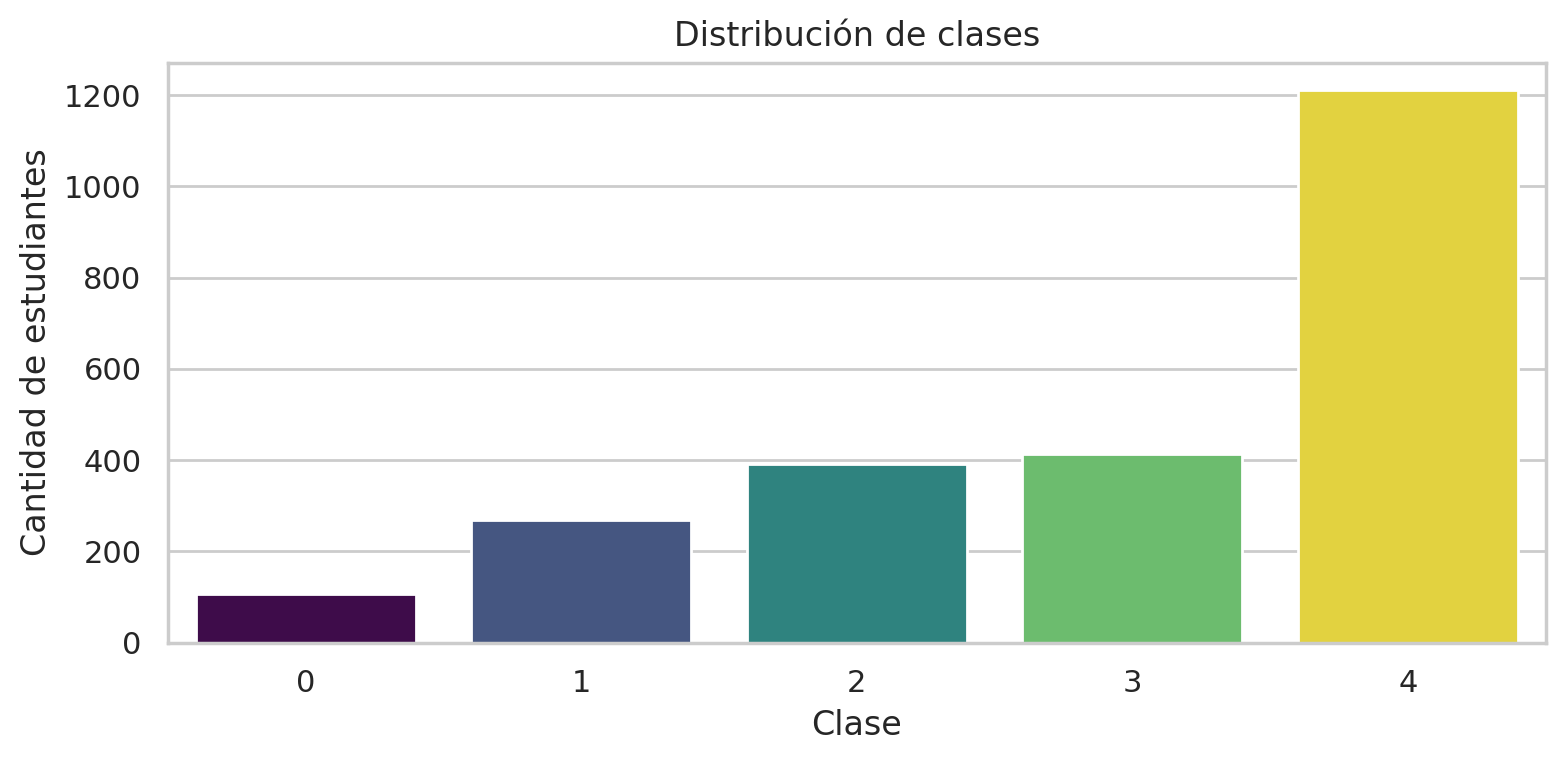
\includegraphics[width=0.9\linewidth]{grafica_distribucion_clases.png}
\caption{Distribución de clases del conjunto de datos.}
\label{fig:clases}
\end{figure}

La Figura~\ref{fig:clases} evidencia el desbalance del dataset: la
clase~4 representa más del 50\% de las muestras, mientras que la
clase~0 es claramente minoritaria con 107 registros. Este desbalance
tiene consecuencias directas sobre el comportamiento de los modelos
y justifica el uso de métricas macro para evaluar el desempeño por
clase de manera equitativa.

\begin{figure}[!t]
\centering
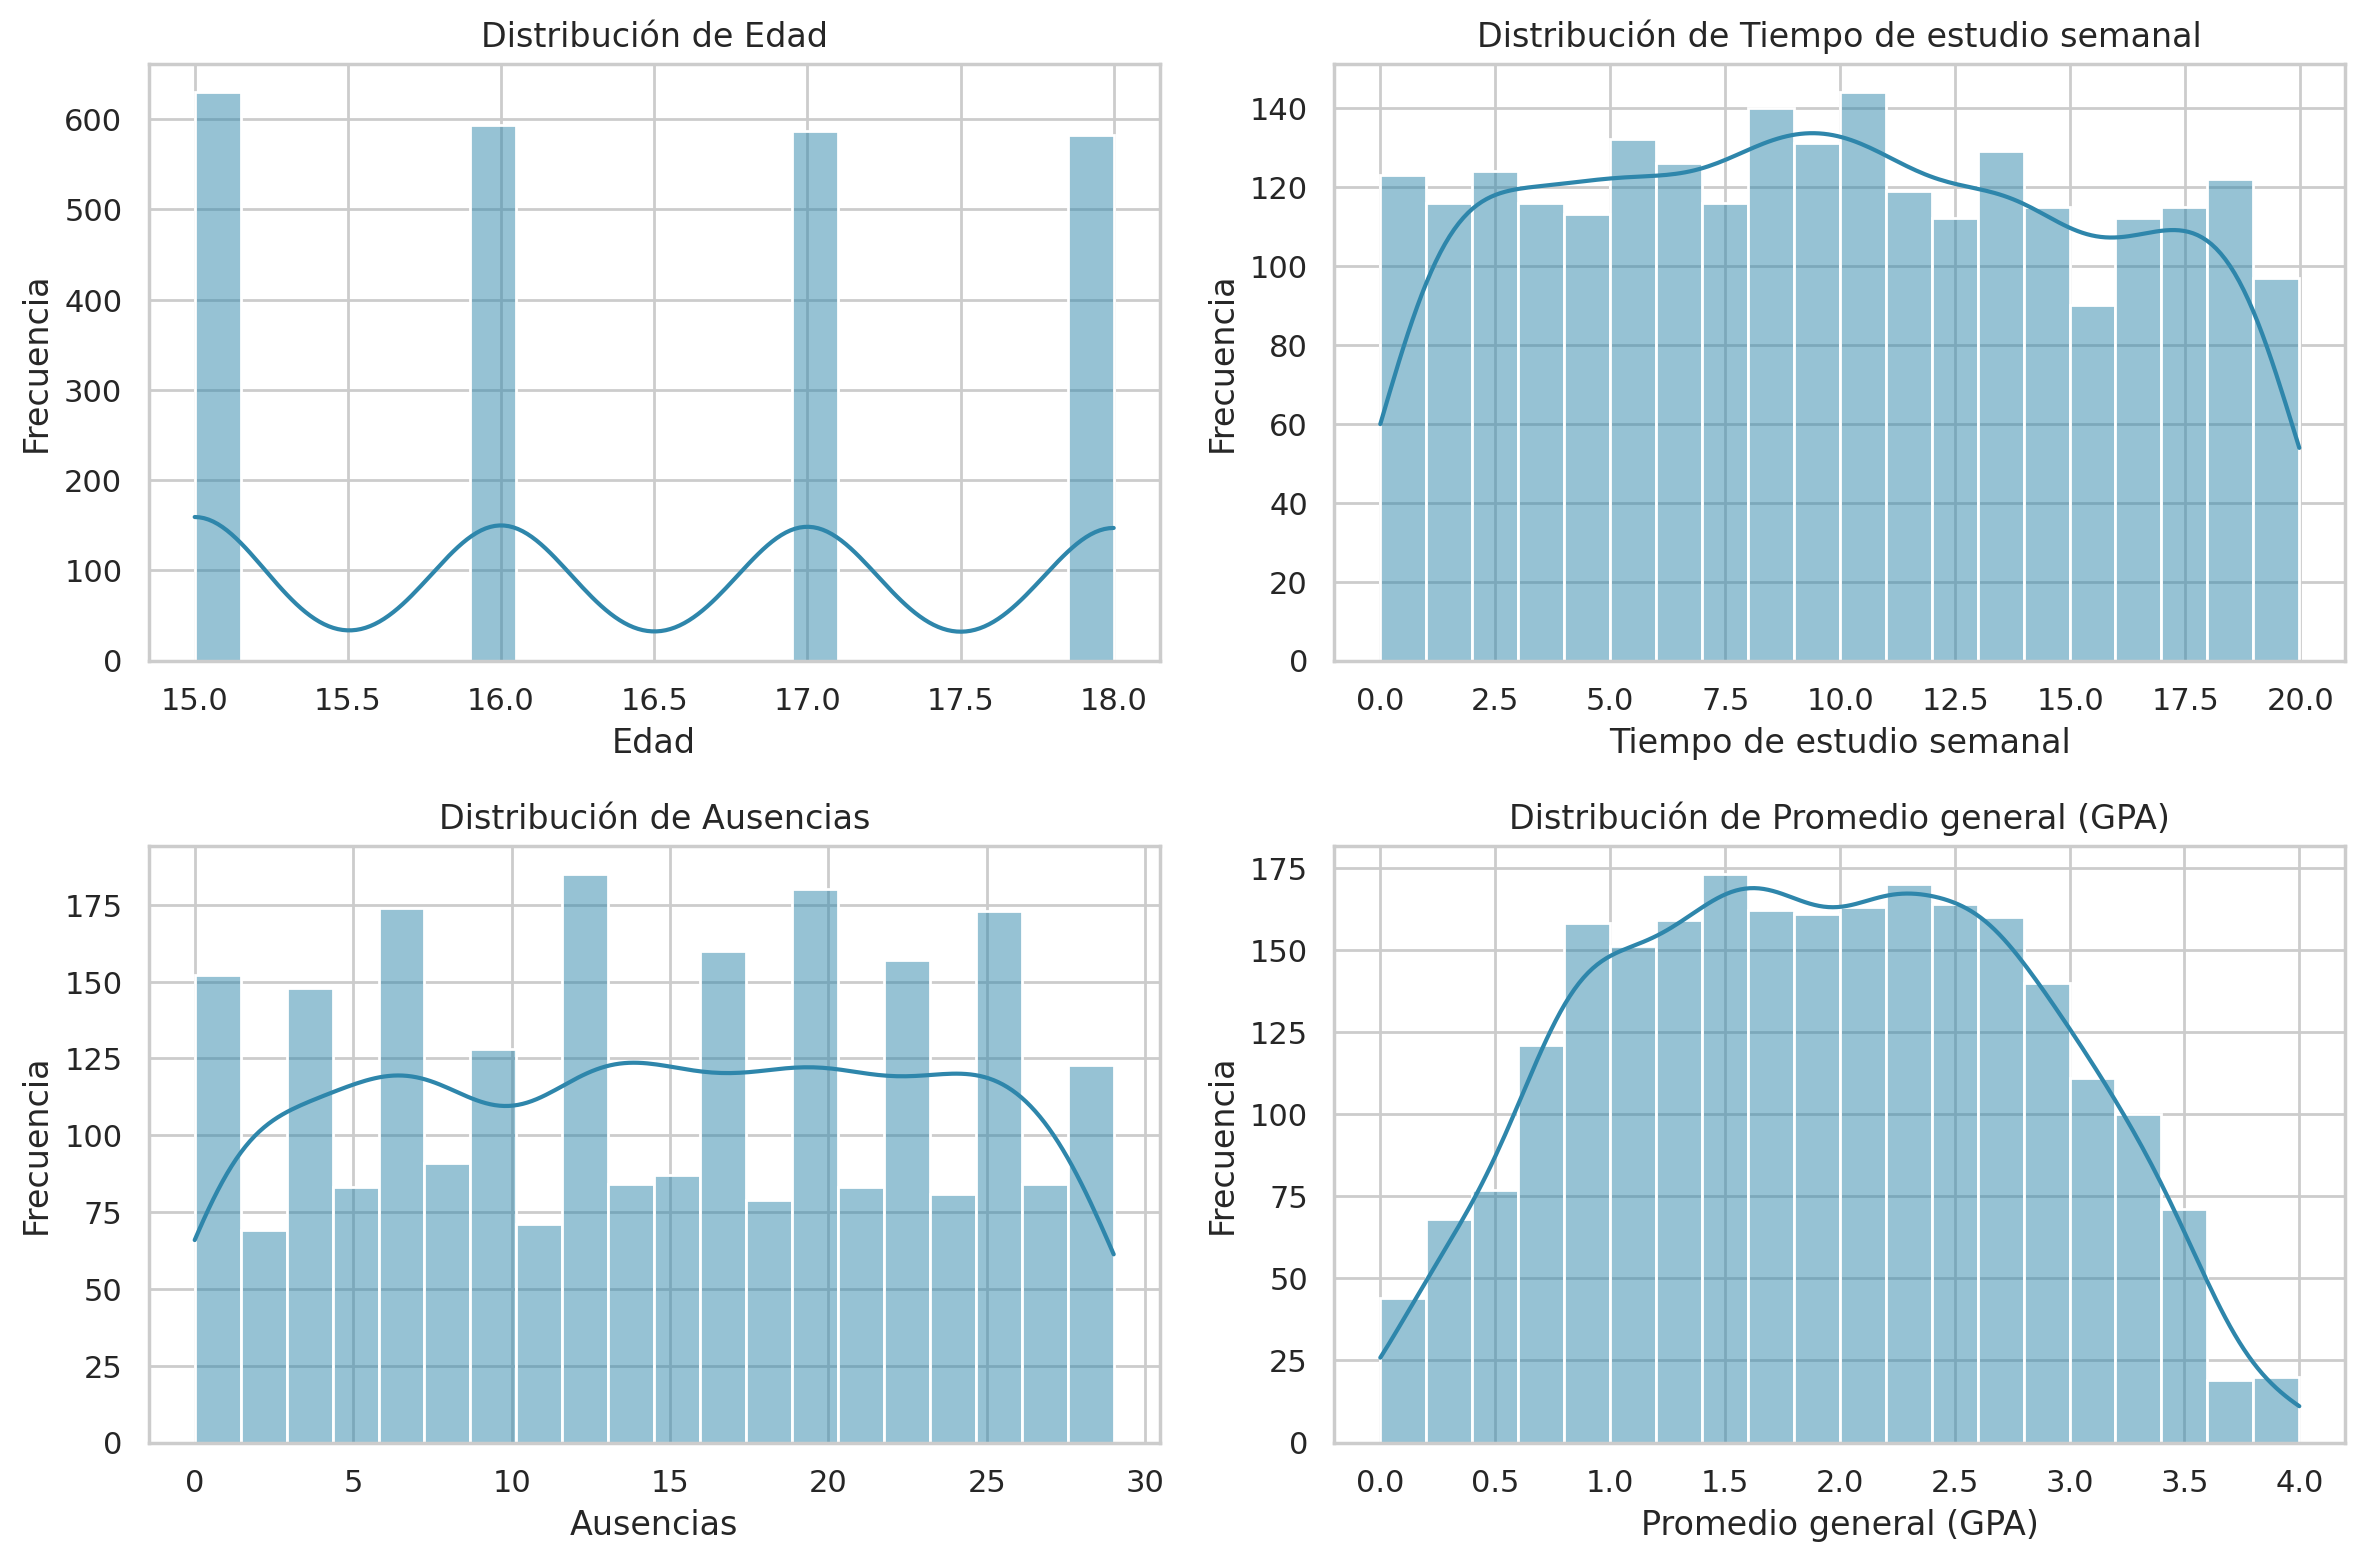
\includegraphics[width=0.95\linewidth]{graficas_distribucion_variables_continuas.png}
\caption{Distribución de las variables continuas utilizadas en el estudio.}
\label{fig:continuas}
\end{figure}

La Figura~\ref{fig:continuas} muestra la distribución de las variables
continuas. La edad presenta un rango muy acotado, lo que anticipa una
baja capacidad discriminativa. El tiempo de estudio semanal, las
ausencias y el promedio general muestran variabilidad más amplia,
sugiriendo mayor potencial explicativo.

\begin{figure}[!t]
\centering
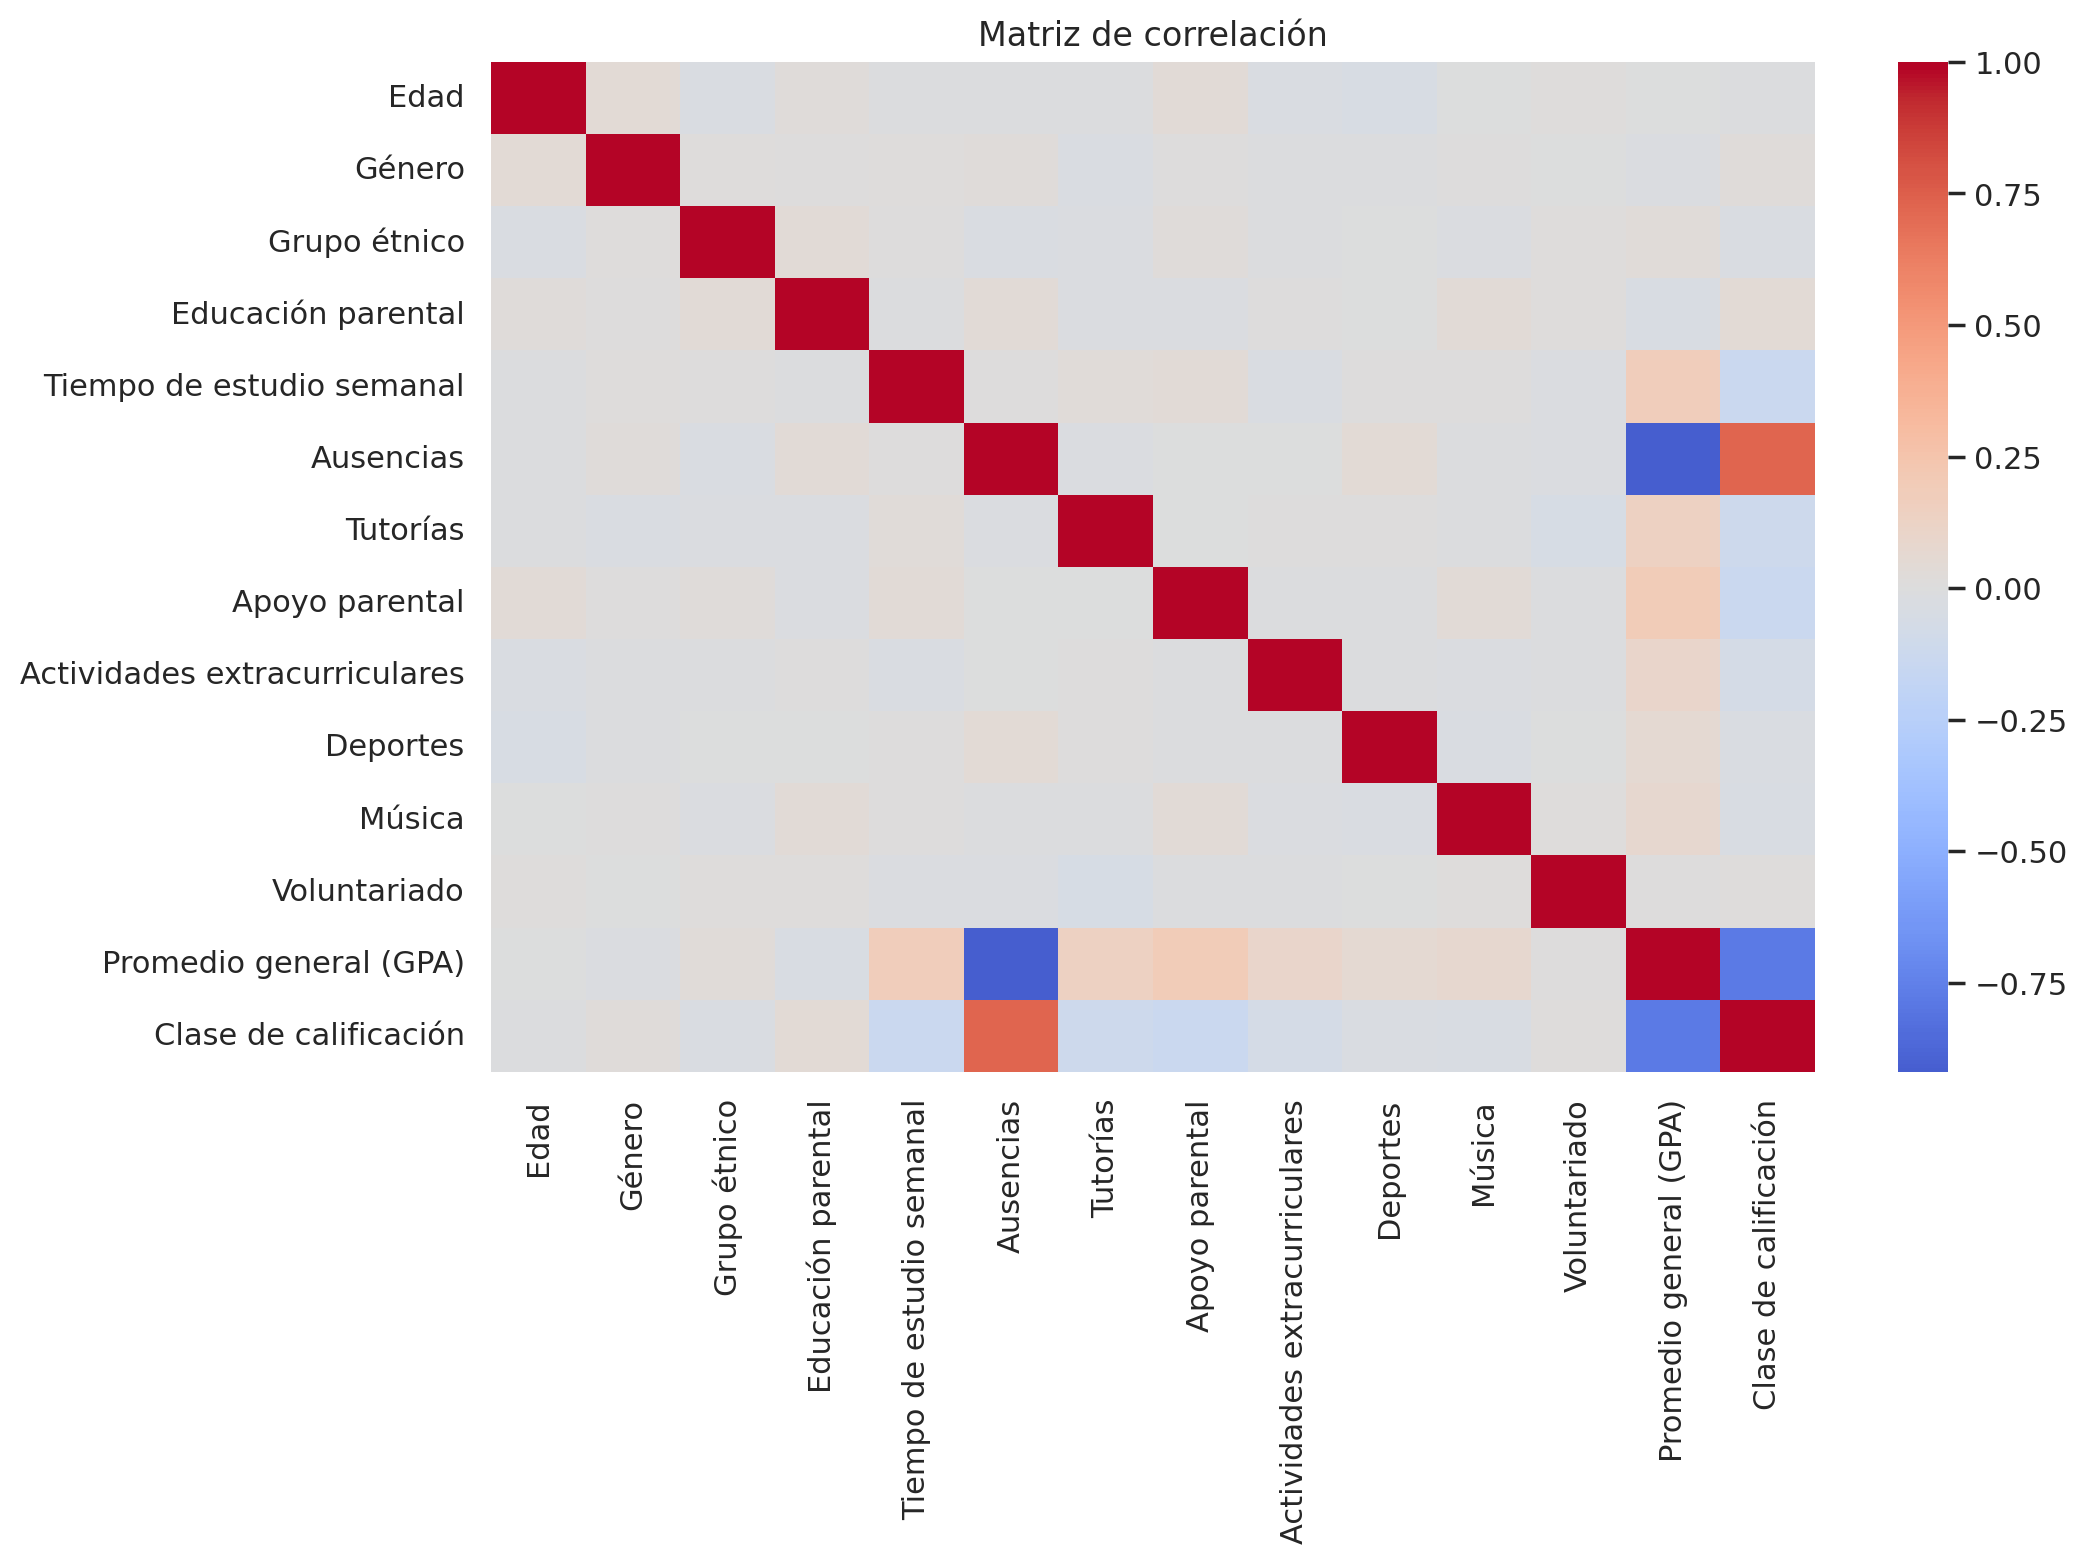
\includegraphics[width=0.95\linewidth]{matriz_correlacion.png}
\caption{Matriz de correlación entre variables.}
\label{fig:corr}
\end{figure}

La Figura~\ref{fig:corr} resume las relaciones lineales entre pares
de variables. Destaca la relación inversa marcada entre \texttt{GPA}
y \texttt{GradeClass}: a mayor promedio general, menor clase numérica,
lo que es coherente con la codificación del problema. Las ausencias
muestran correlación positiva con la clase de calificación, indicando
que mayor ausentismo se asocia con peor desempeño.

\begin{figure}[!t]
\centering
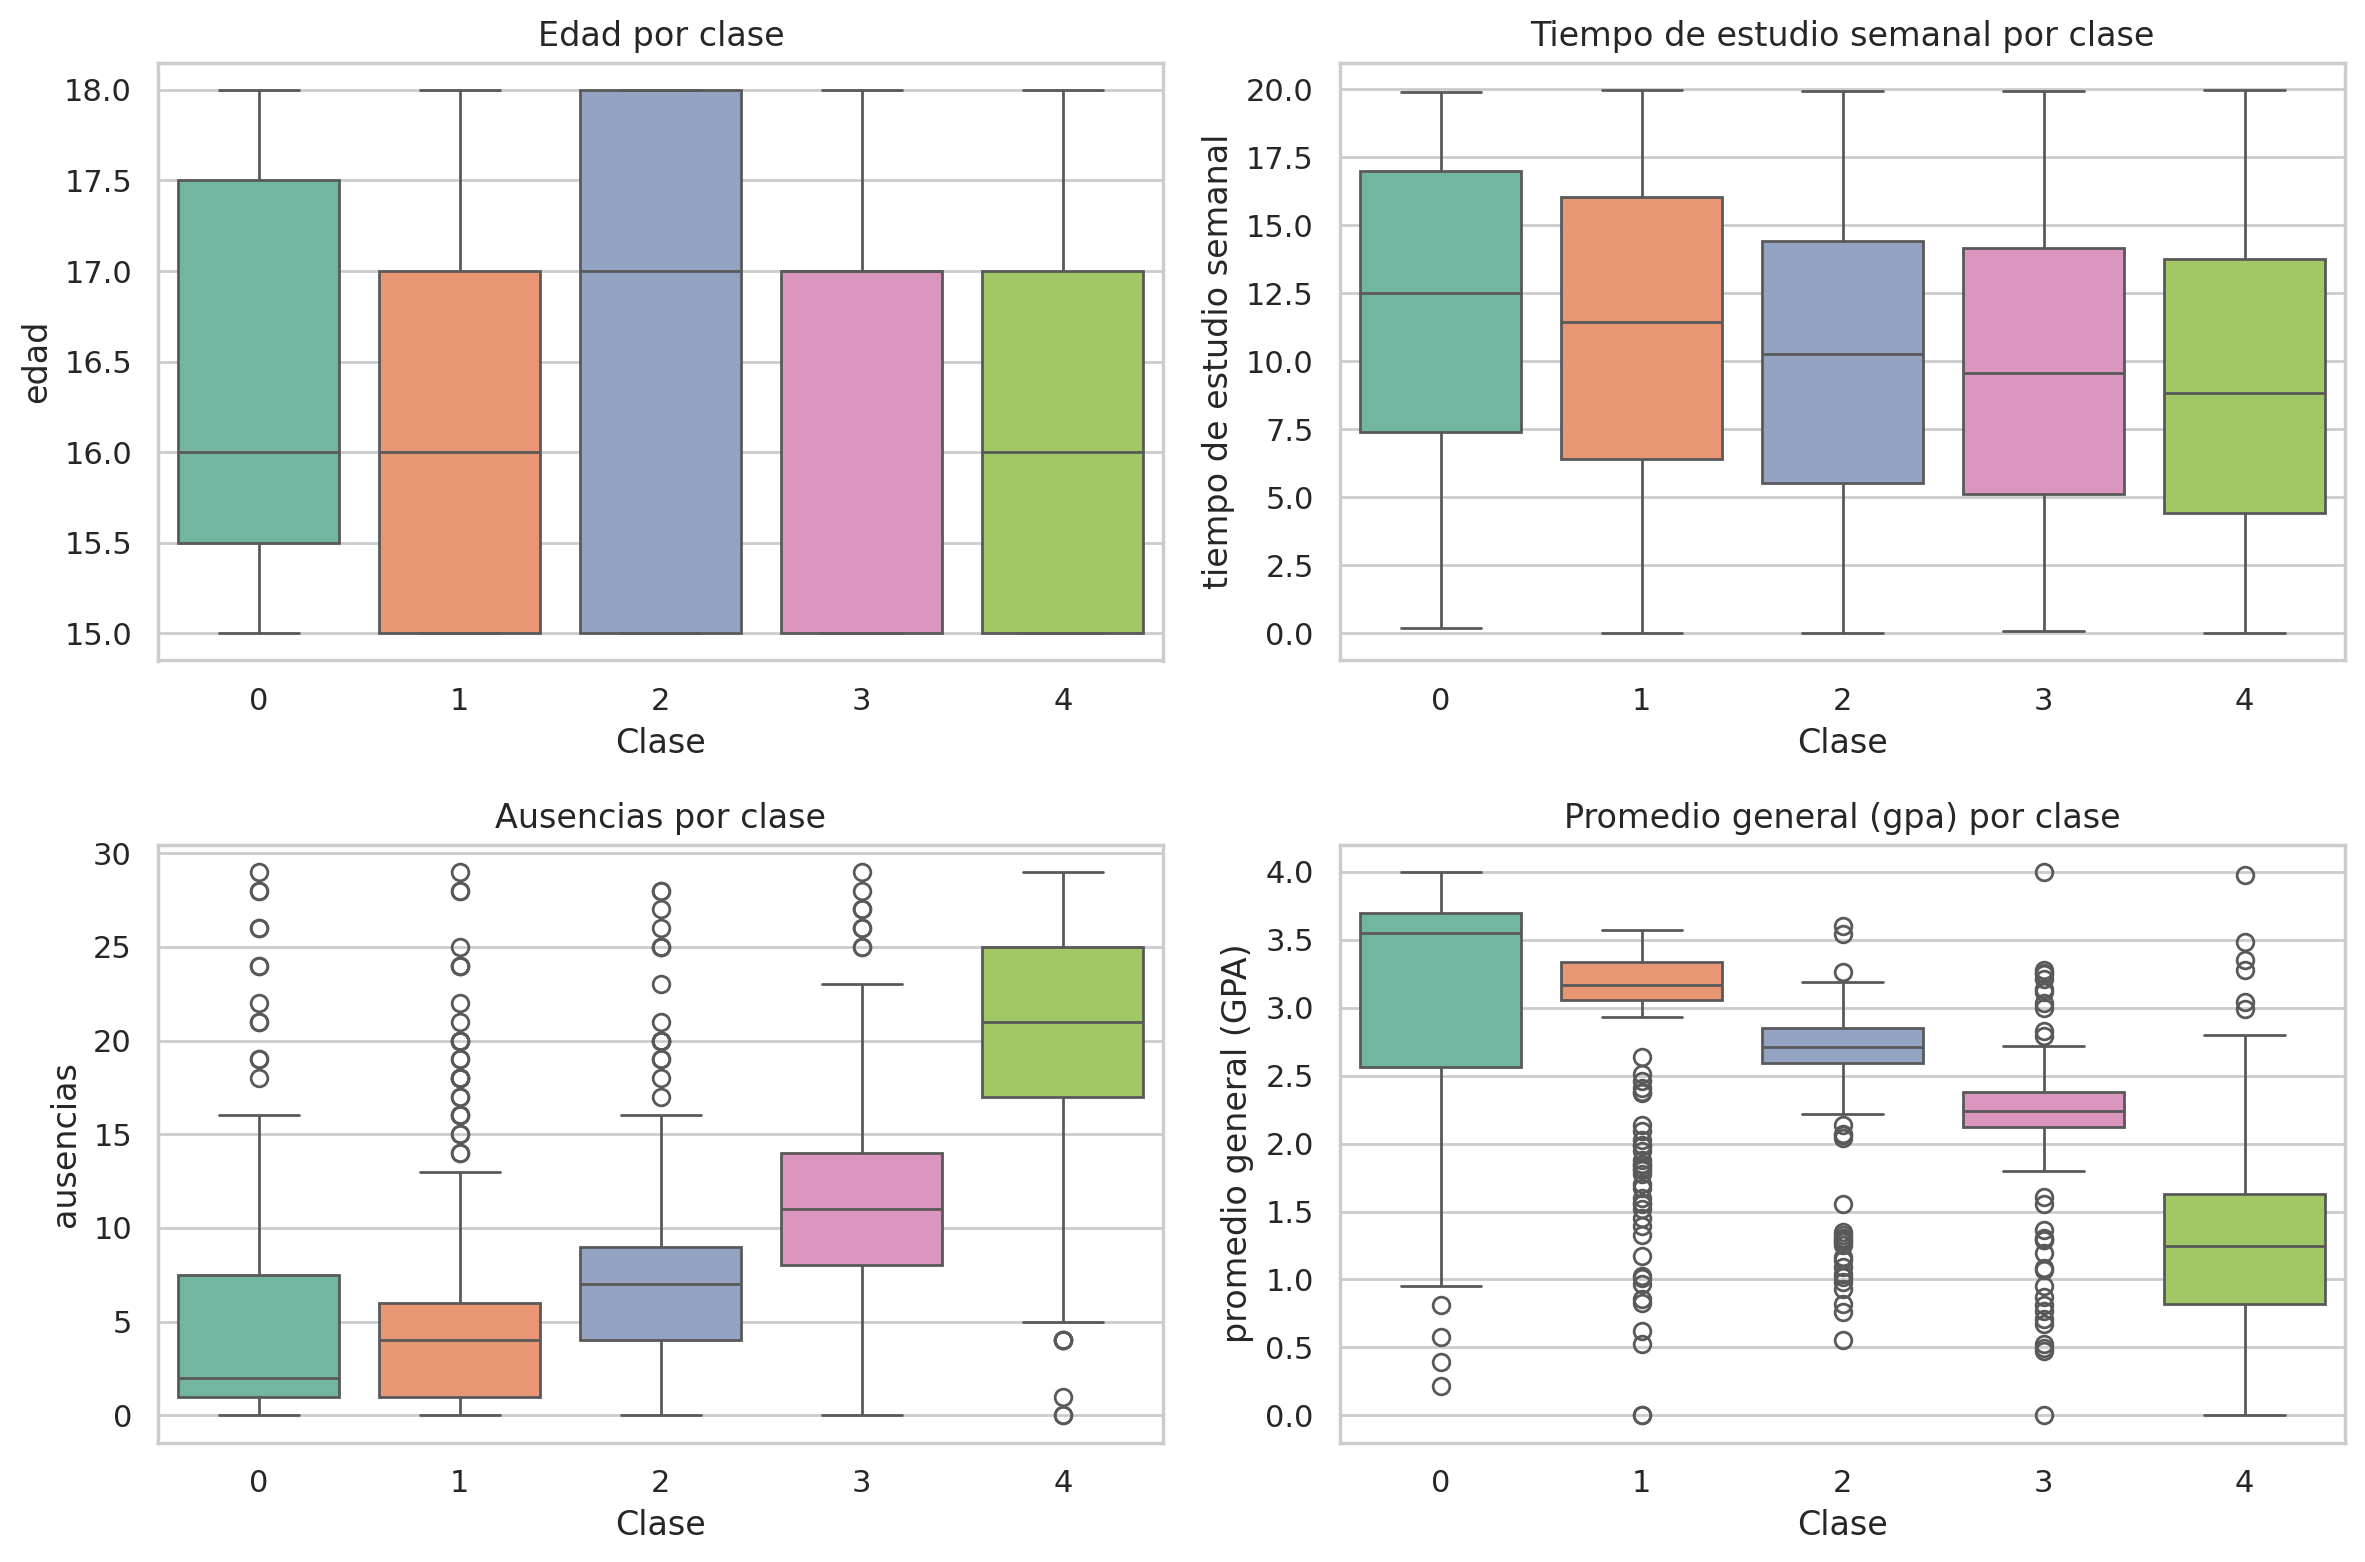
\includegraphics[width=0.95\linewidth]{boxplots_variables_por_clase.png}
\caption{Distribución de variables continuas por clase mediante diagramas de caja.}
\label{fig:boxplots}
\end{figure}

La Figura~\ref{fig:boxplots} complementa la matriz de correlación al
mostrar cómo cambian la mediana y la dispersión de cada variable
continua a lo largo de las clases. Las ausencias aumentan
progresivamente conforme empeora la clase, mientras que el promedio
general disminuye. La edad permanece estable entre clases, confirmando
su baja capacidad discriminativa.

\begin{figure}[!t]
\centering
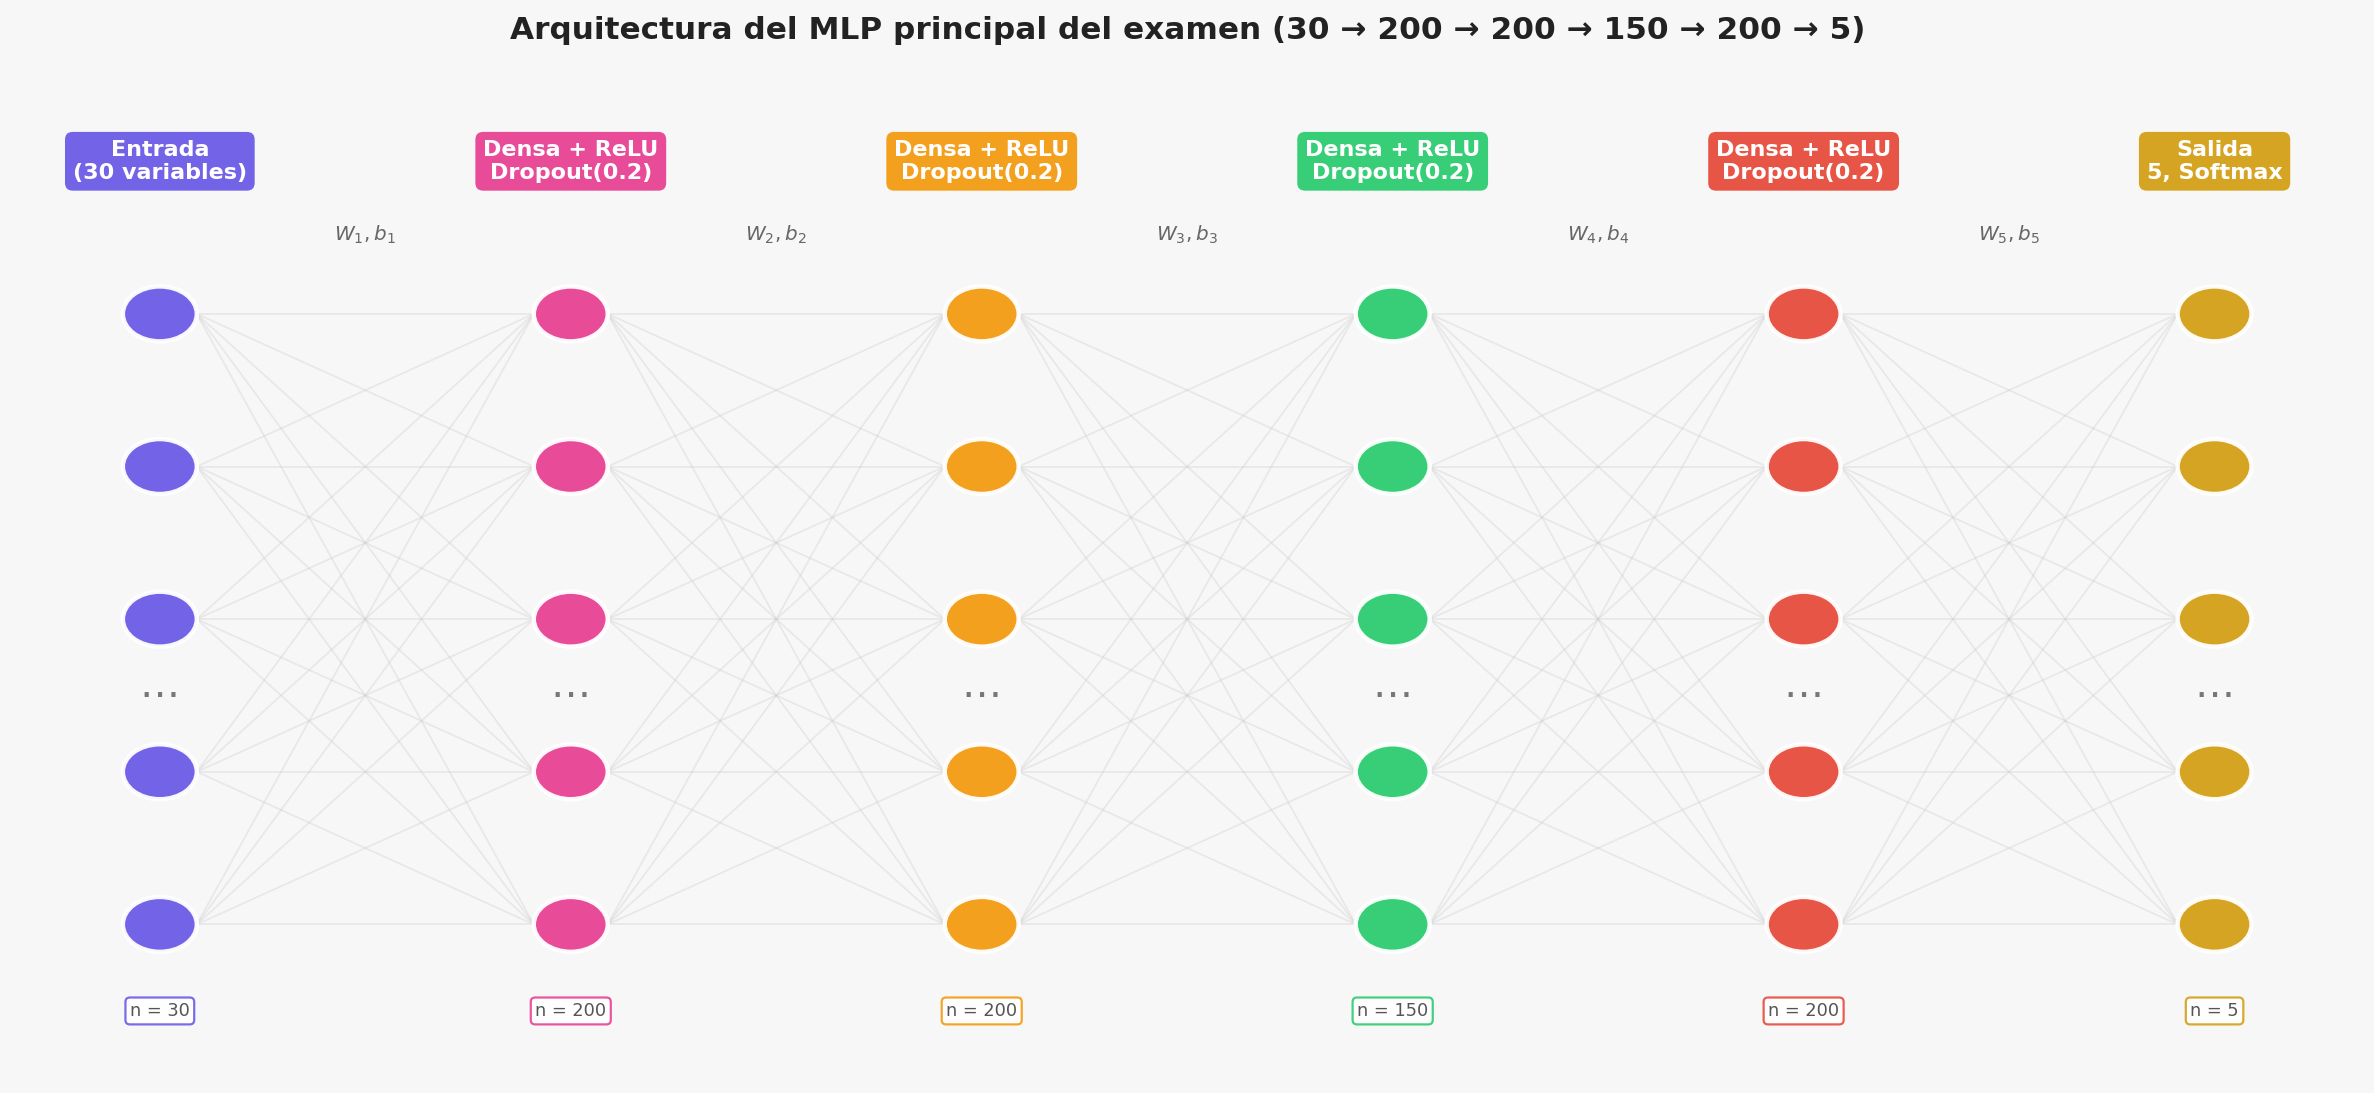
\includegraphics[width=0.95\linewidth]{arquitectura_mlp_principal.png}
\caption{Arquitectura del MLP principal utilizada en el experimento.}
\label{fig:mlp}
\end{figure}

La Figura~\ref{fig:mlp} representa visualmente la arquitectura del
modelo principal: capa de entrada, cuatro capas densas con activación
ReLU y \textit{Dropout}(0.2), y capa de salida con cinco neuronas y
activación \textit{softmax}.

\begin{figure}[!t]
\centering
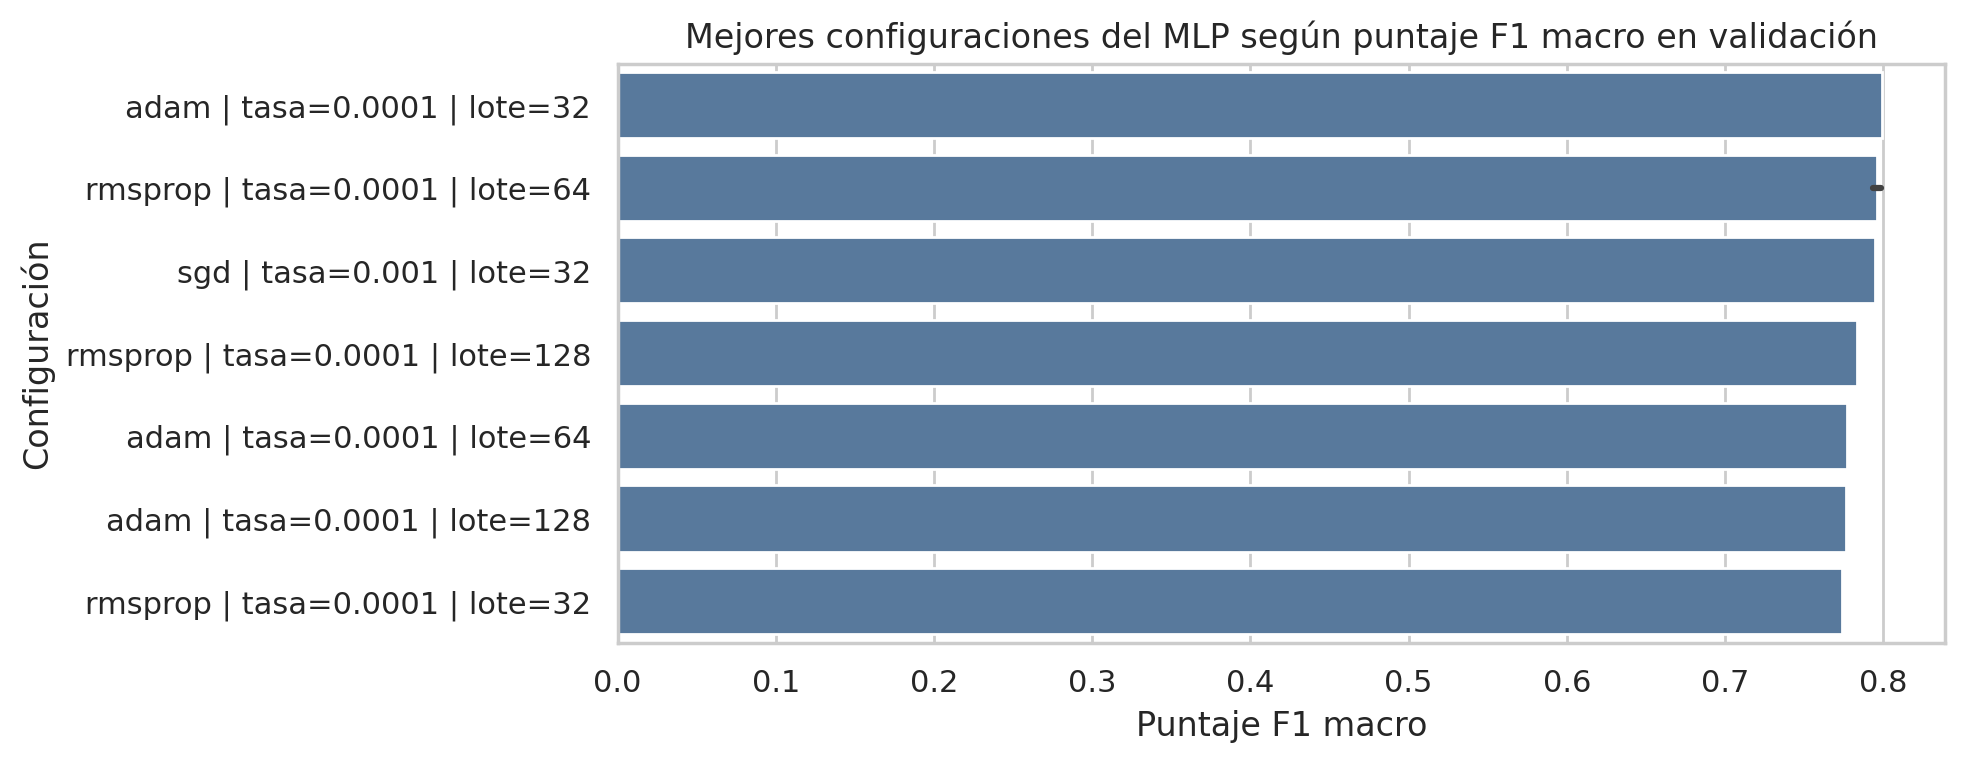
\includegraphics[width=0.95\linewidth]{comparacion_hiperparametros_mlp.png}
\caption{Comparación de hiperparámetros evaluados para el MLP principal.}
\label{fig:busqueda_mlp}
\end{figure}

La Figura~\ref{fig:busqueda_mlp} documenta la exploración de
hiperparámetros del MLP. Se observa que las configuraciones con
\texttt{Adam} y tasa de aprendizaje de 0.0001 concentran los mejores
valores de F1 macro en validación, mientras que \texttt{SGD} con
tasas más altas presenta mayor variabilidad en los resultados.

\begin{figure}[!t]
\centering
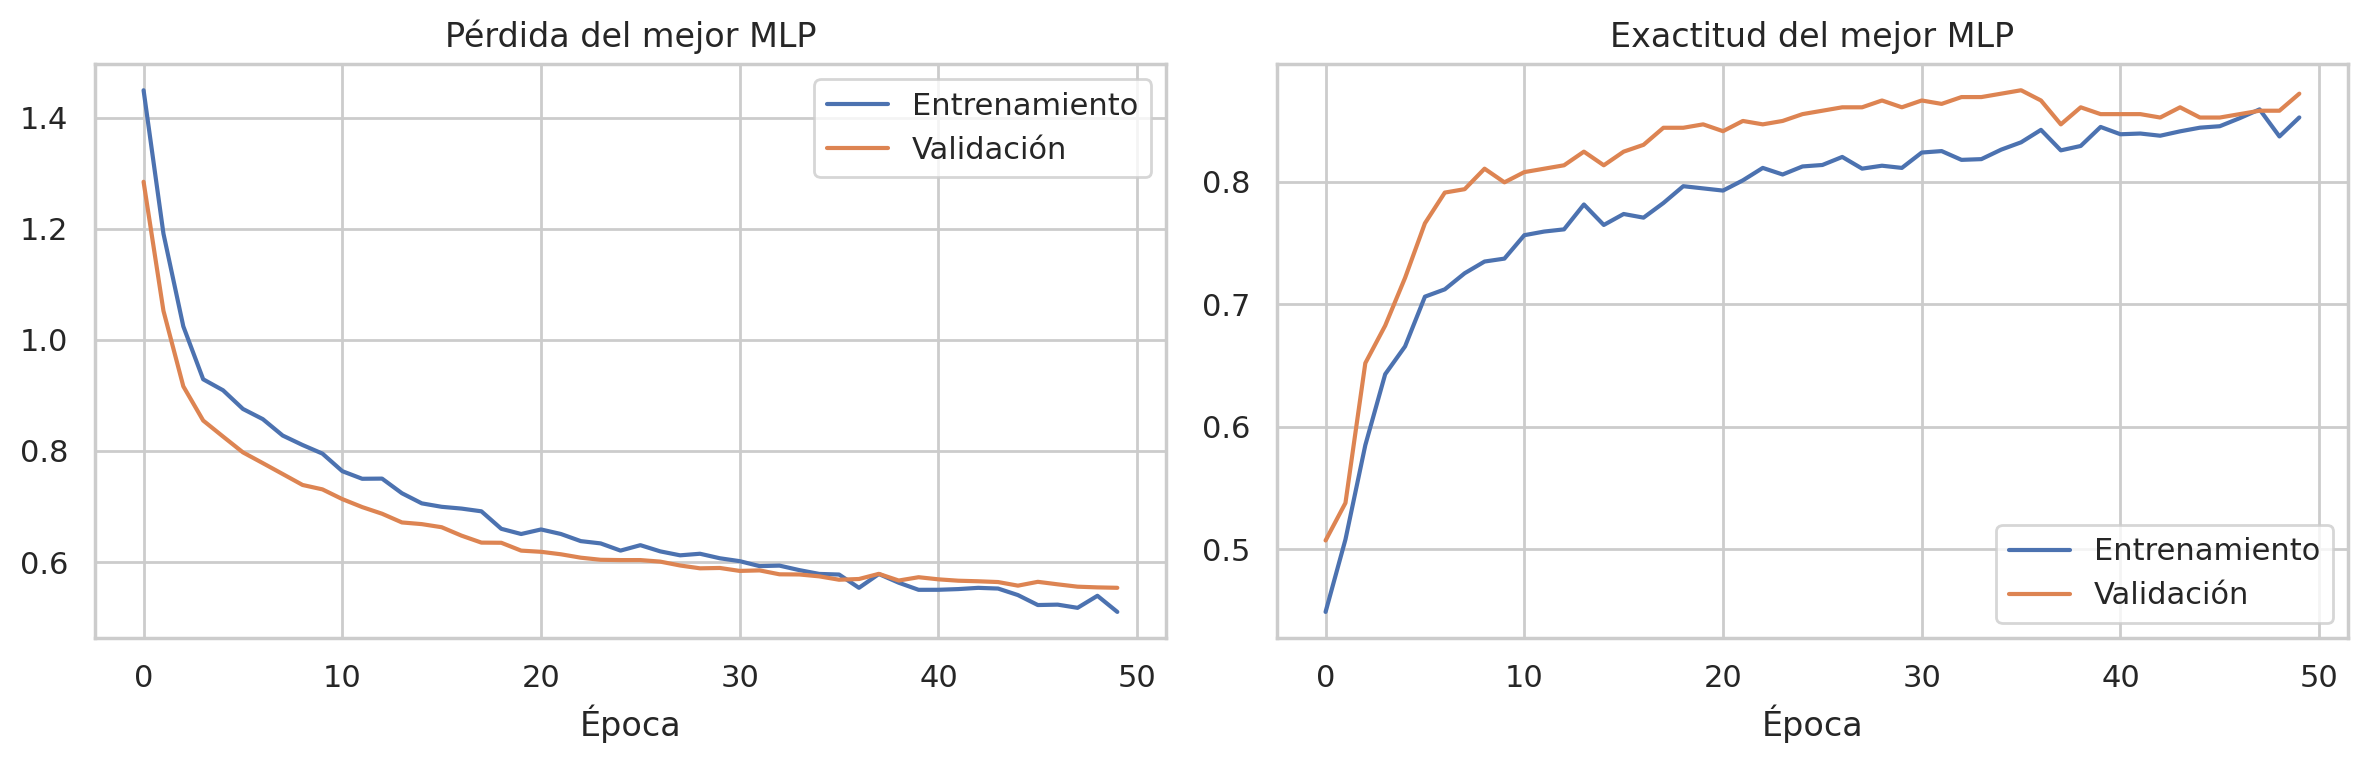
\includegraphics[width=0.95\linewidth]{curvas_entrenamiento_mlp.png}
\caption{Curvas de pérdida y exactitud del mejor MLP durante entrenamiento y validación.}
\label{fig:curvas_mlp}
\end{figure}

La Figura~\ref{fig:curvas_mlp} muestra la evolución del aprendizaje
del mejor MLP. En la curva de pérdida se observa una disminución
consistente en ambos subconjuntos, sin divergencia entre entrenamiento
y validación. La curva de exactitud confirma una mejora sostenida y
estable. La proximidad entre ambas curvas sugiere que el
\textit{Dropout} cumplió su función regulatoria de manera efectiva.

\begin{figure}[!t]
\centering
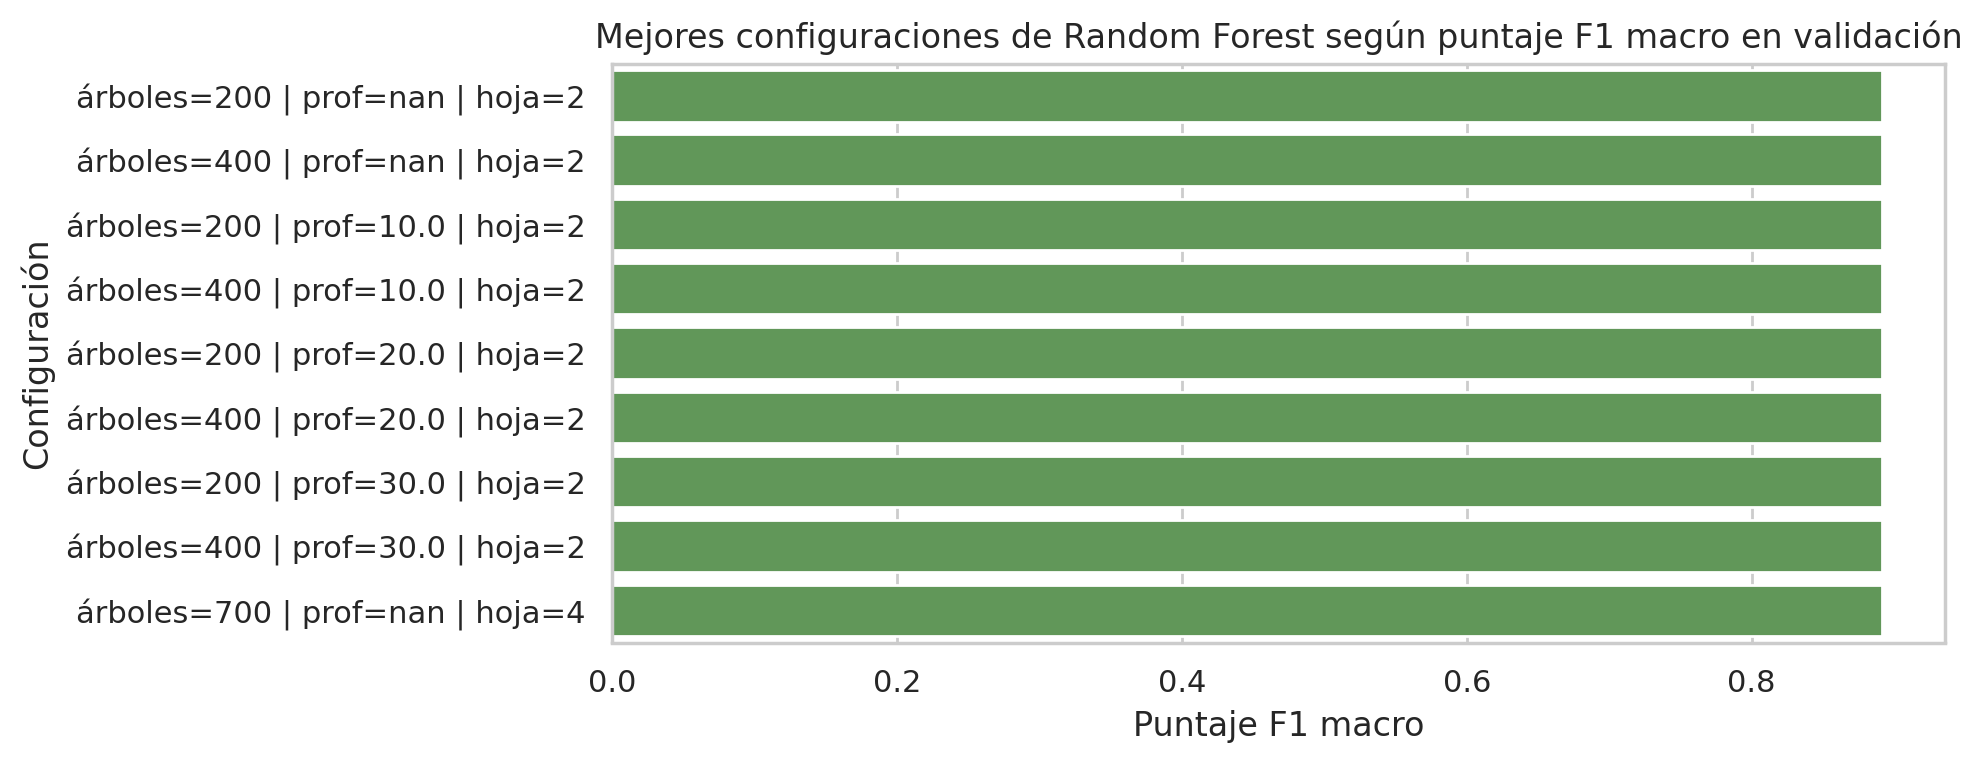
\includegraphics[width=0.95\linewidth]{comparacion_hiperparametros_random_forest.png}
\caption{Comparación de hiperparámetros evaluados para Random Forest.}
\label{fig:busqueda_rf}
\end{figure}

La Figura~\ref{fig:busqueda_rf} presenta la exploración de
hiperparámetros de \textit{Random Forest}. Las configuraciones con
profundidad sin límite y tamaños mínimos de hoja pequeños tienden a
concentrar los mejores resultados, aunque con diferencias marginales
entre ellas.

\begin{table}[!t]
\centering
\caption{Comparación final de modelos}
\scriptsize
\setlength{\tabcolsep}{4pt}
\begin{tabular}{p{2.2cm}cccc}
\toprule
Modelo & Exactitud & Precisión macro & Sensibilidad macro & Puntaje F1 macro \\
\midrule
MLP principal  & 0.8607 & 0.8270 & 0.7405 & 0.7643 \\
Random Forest  & 0.9331 & 0.9147 & 0.8363 & 0.8604 \\
\bottomrule
\end{tabular}
\normalsize
\label{tab:comparacion}
\end{table}

La Tabla~\ref{tab:comparacion} concentra la comparación cuantitativa
principal. El MLP alcanzó una exactitud de 0.8607 y un puntaje F1
macro de 0.7643, resultado sólido considerando la arquitectura fija
requerida. \textit{Random Forest} superó al MLP en todas las métricas,
alcanzando 0.9331 de exactitud y 0.8604 de F1 macro.

\begin{figure}[!t]
\centering
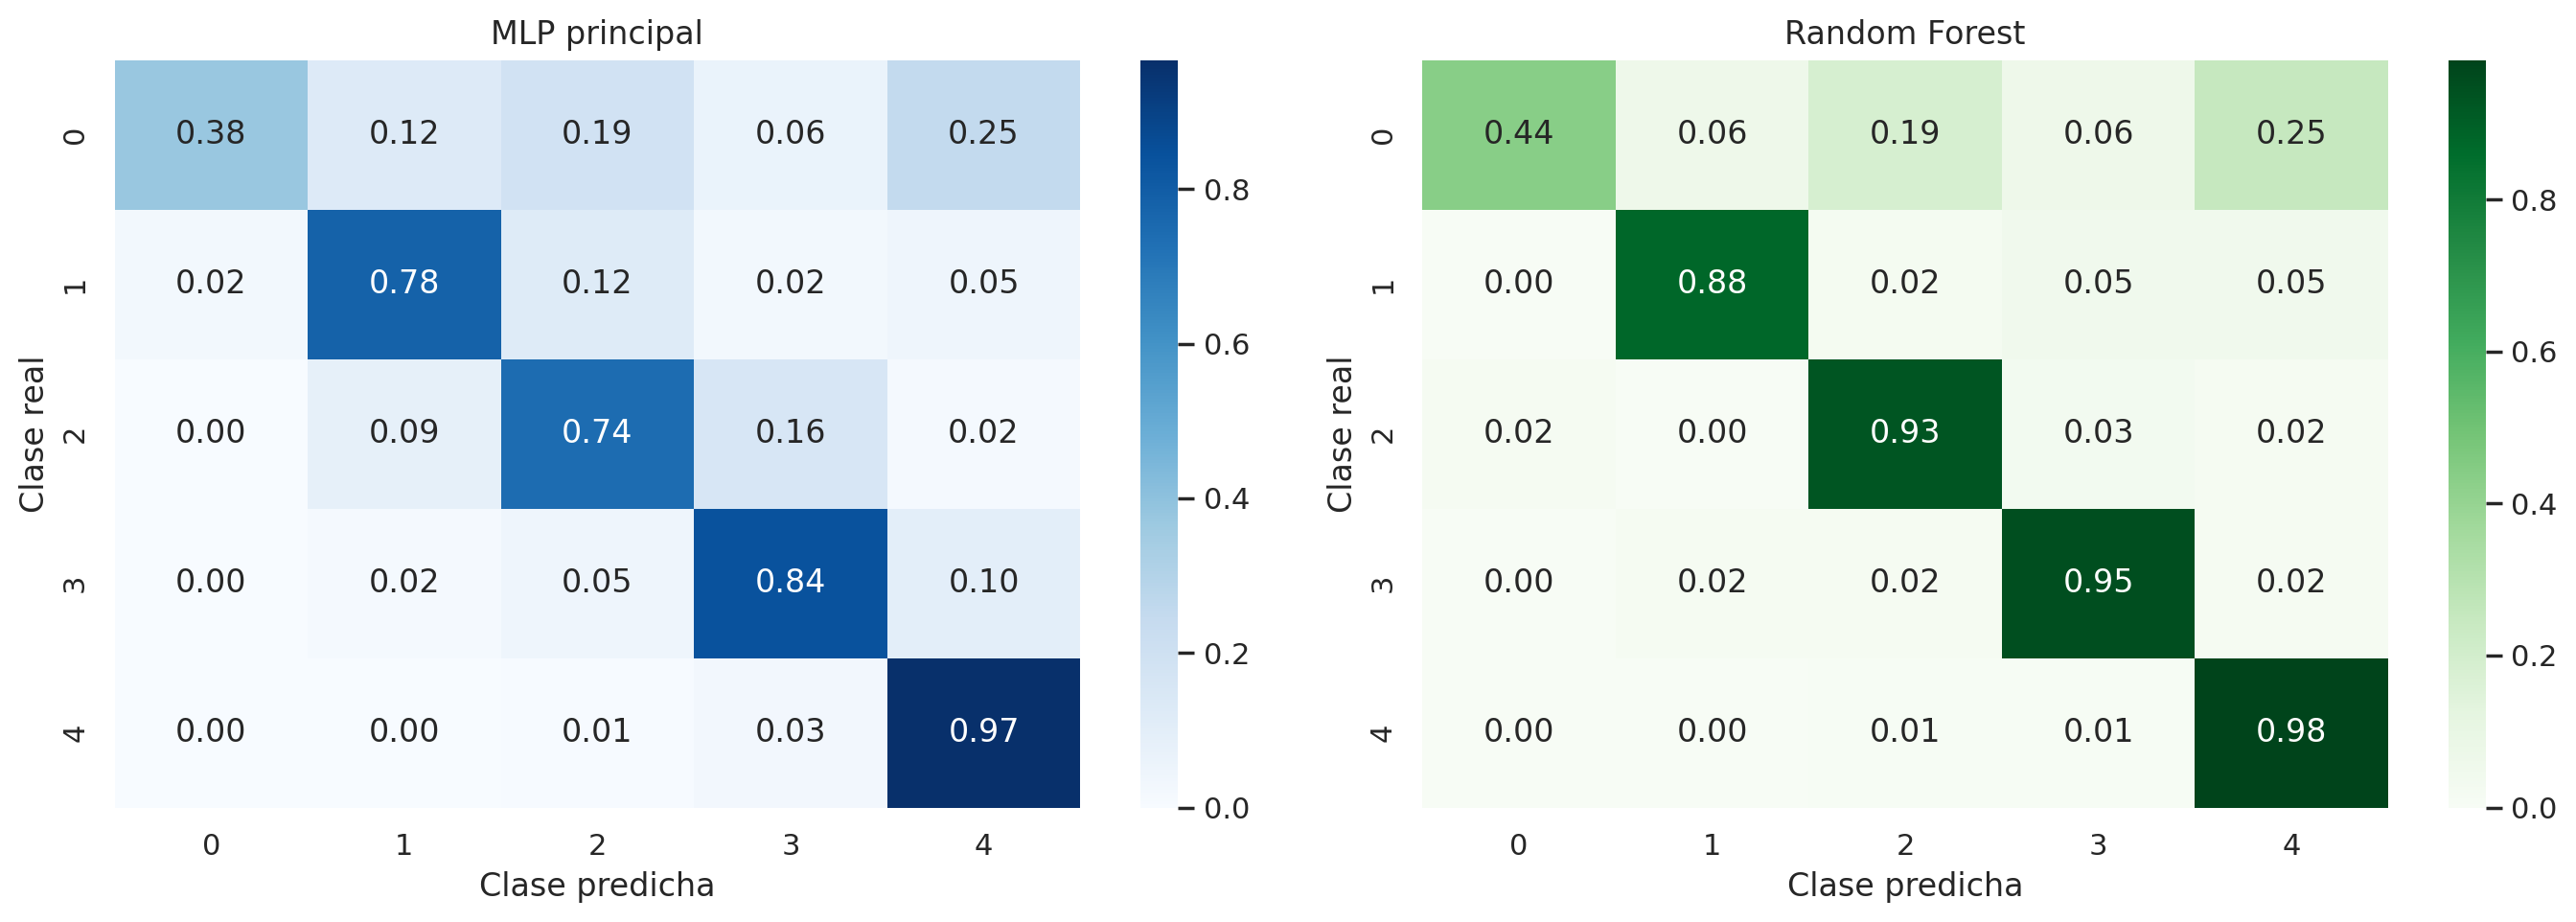
\includegraphics[width=0.95\linewidth]{matrices_confusion_comparadas.png}
\caption{Matrices de confusión normalizadas del MLP principal y de Random Forest.}
\label{fig:confusiones}
\end{figure}

La Figura~\ref{fig:confusiones} revela la estructura de errores de
cada modelo. En ambos casos la clase~4 obtiene el mejor
reconocimiento, asociado tanto a su mayor frecuencia como a la
señal explicativa de \texttt{GPA}. La clase~0 es la más difícil
en ambos modelos, aunque \textit{Random Forest} logra una tasa de
identificación superior. Los errores se concentran principalmente
entre clases adyacentes, lo que es coherente con la naturaleza
ordinal del problema.

\begin{figure}[!t]
\centering
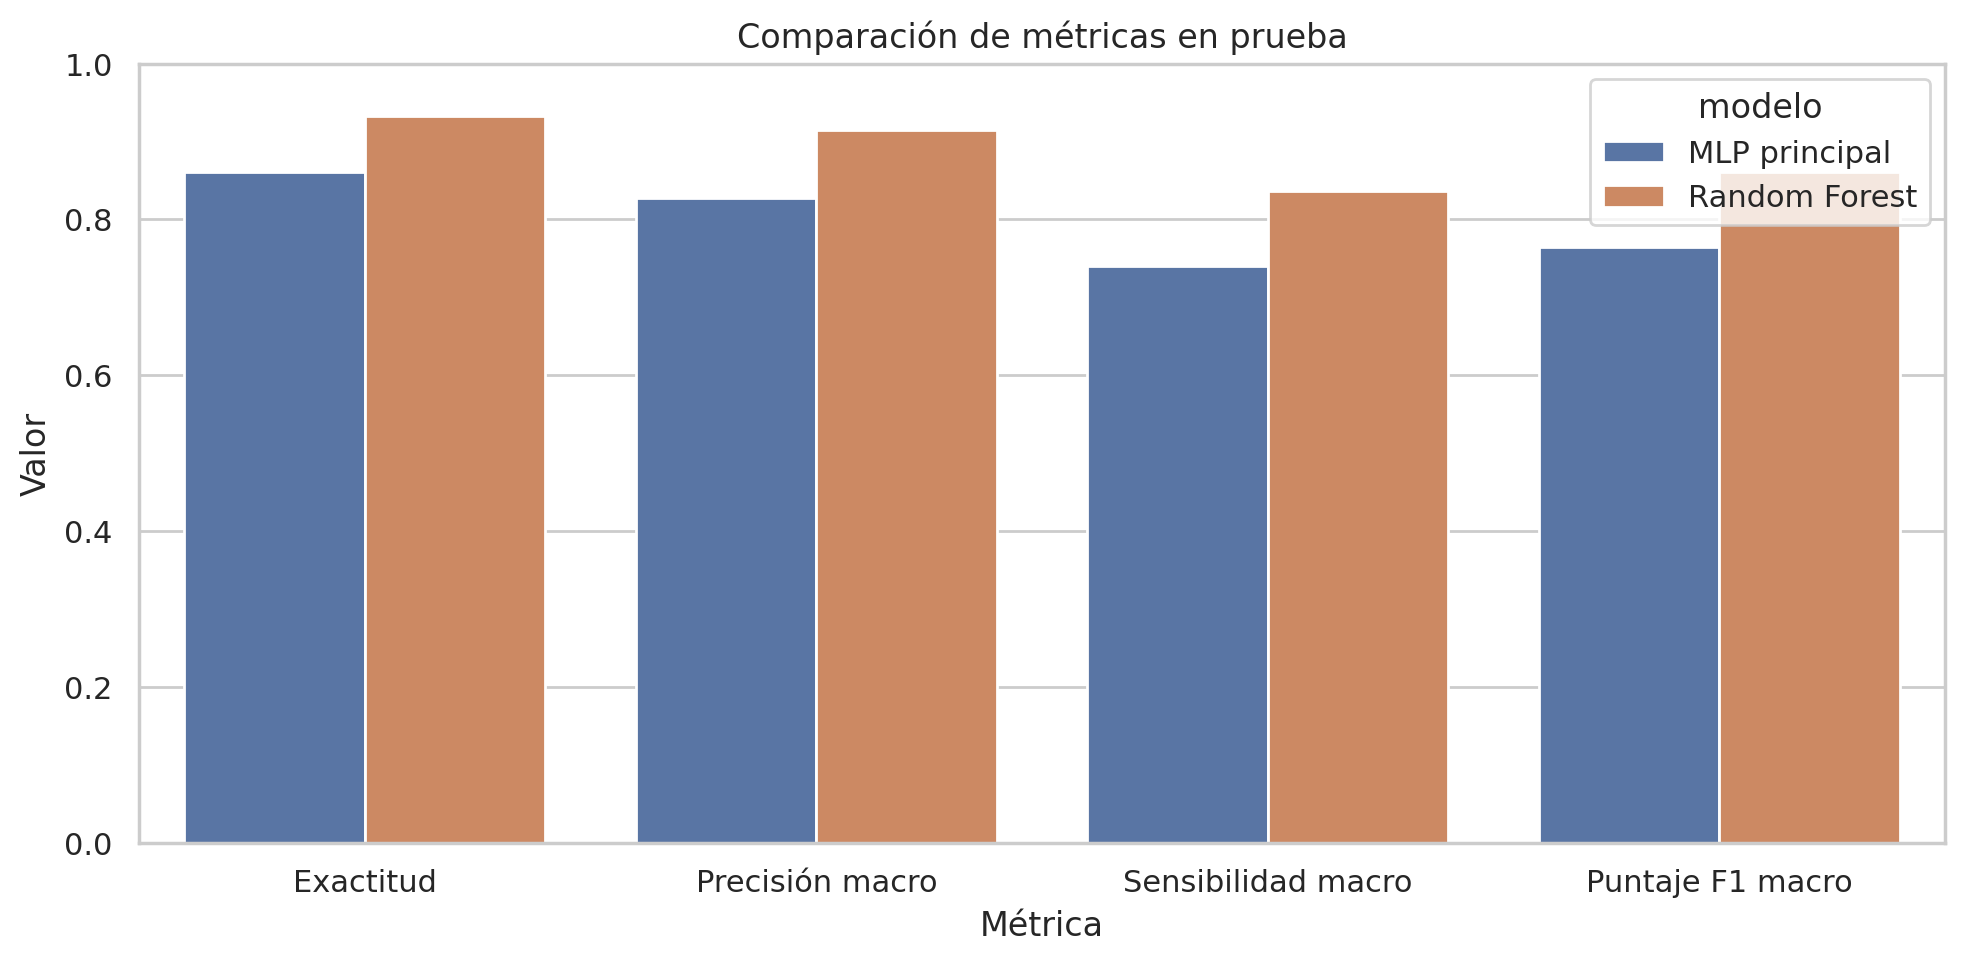
\includegraphics[width=0.95\linewidth]{comparacion_metricas_modelos.png}
\caption{Comparación de métricas entre modelos.}
\label{fig:metricas}
\end{figure}

La Figura~\ref{fig:metricas} facilita la lectura comparativa del
desempeño. Confirma visualmente que la ventaja de \textit{Random
Forest} sobre el MLP es consistente en exactitud, precisión macro,
sensibilidad macro y puntaje F1 macro, y no se limita a una sola
métrica.

\begin{figure}[!t]
\centering
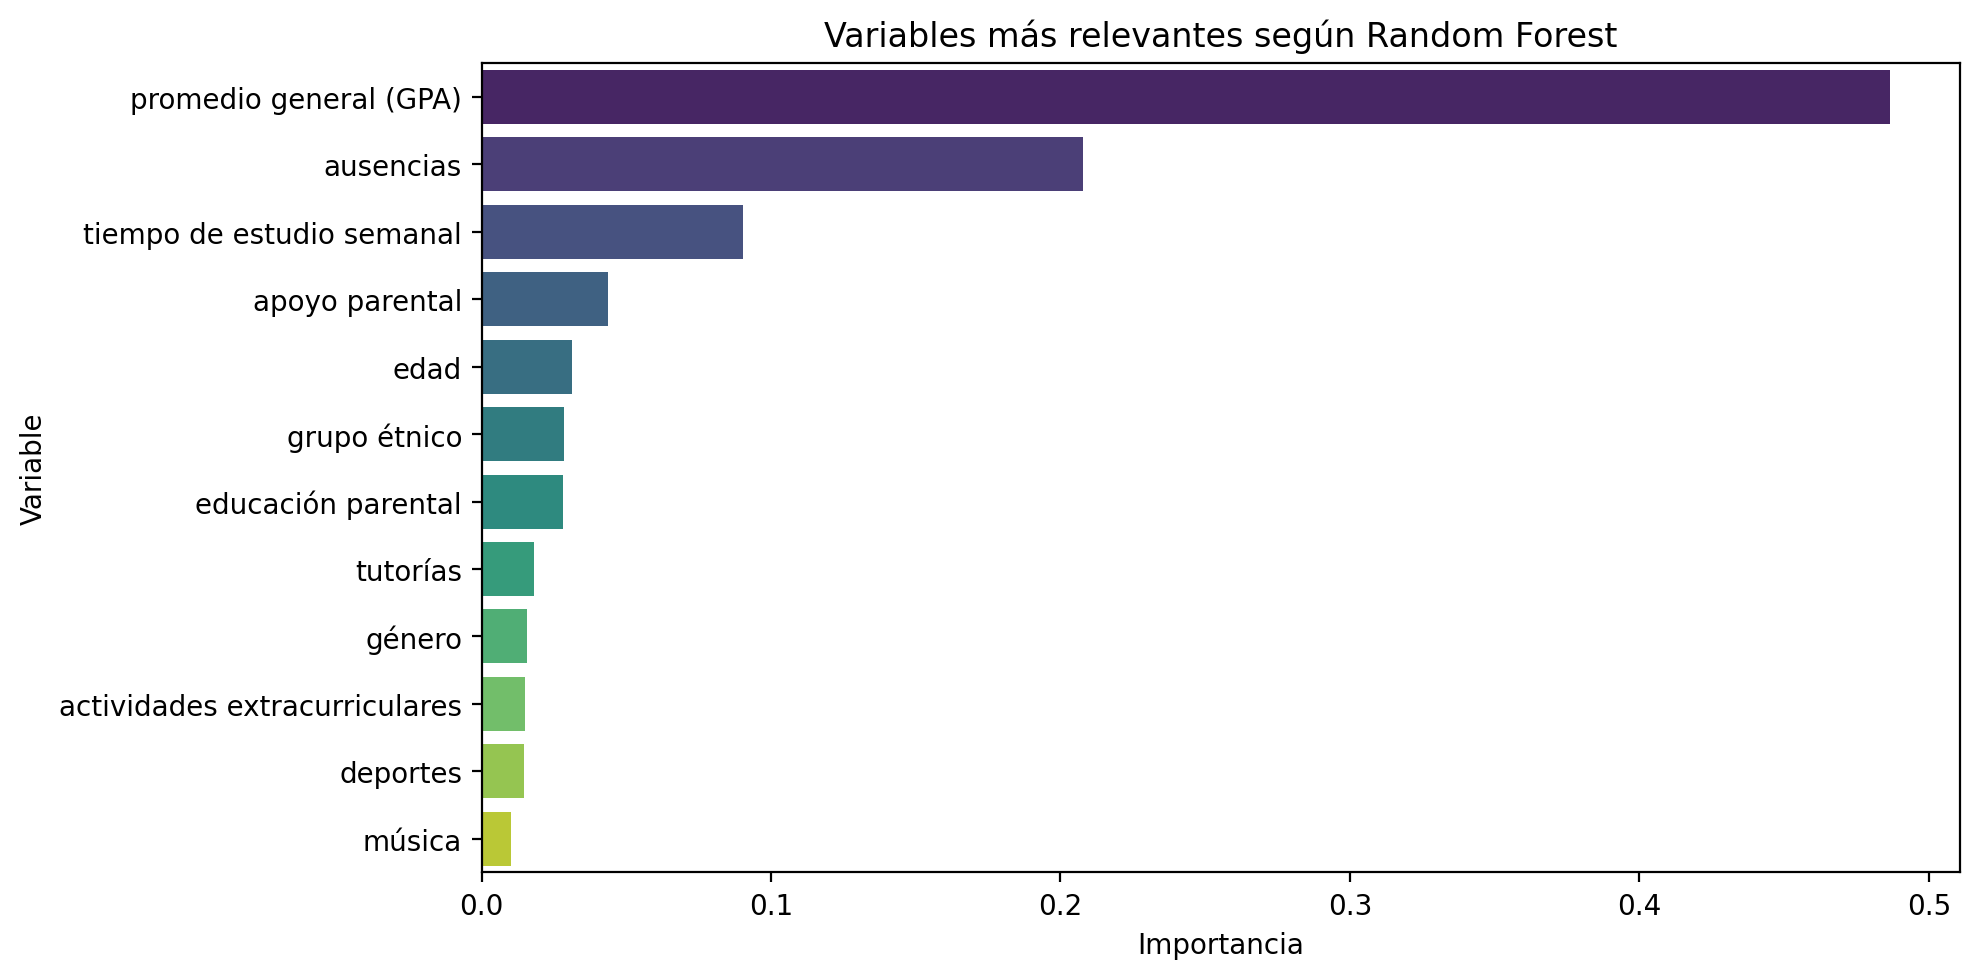
\includegraphics[width=0.95\linewidth]{importancia_variables_random_forest.png}
\caption{Importancia de variables estimada por Random Forest.}
\label{fig:importancia}
\end{figure}

\begin{table}[!t]
\centering
\caption{Variables más relevantes según Random Forest}
\scriptsize
\setlength{\tabcolsep}{5pt}
\begin{tabular}{lc}
\toprule
Variable & Importancia \\
\midrule
GPA                        & 0.4864 \\
ausencias                  & 0.2076 \\
tiempo de estudio semanal  & 0.0904 \\
apoyo parental             & 0.0437 \\
edad                       & 0.0311 \\
grupo étnico               & 0.0285 \\
educación parental         & 0.0281 \\
\bottomrule
\end{tabular}
\normalsize
\label{tab:importancia}
\end{table}

La Figura~\ref{fig:importancia} y la Tabla~\ref{tab:importancia}
muestran que \texttt{GPA} es, por amplio margen, la variable más
influyente (0.4864), seguida por las ausencias (0.2076) y el tiempo
de estudio semanal (0.0904). Variables como la edad, el grupo étnico
y la educación parental contribuyen de forma marginal. Estos resultados
son coherentes con la semántica del problema: el desempeño pasado y
los hábitos de dedicación escolar son los predictores más directos
de la clase de calificación.

\section{Discusión}\label{sec:discusion}

El MLP principal alcanzó una exactitud de 0.8607 y un F1 macro de
0.7643, confirmando que la arquitectura especificada en el enunciado
es capaz de resolver el problema de manera competitiva. La búsqueda
de hiperparámetros mostró que la configuración óptima (\texttt{Adam},
tasa 0.0001, lote 32, 50 épocas) favoreció un aprendizaje gradual y
estable, visible en las curvas de la Figura~\ref{fig:curvas_mlp}.

\textit{Random Forest} superó al MLP en todas las métricas principales.
Este resultado es coherente con la literatura para problemas educativos
con datos tabulares, donde los métodos de ensamble suelen superar a
arquitecturas profundas cuando el dataset es relativamente compacto y
contiene variables altamente informativas~\cite{rf_algorithms,rf_dropout_review,rf_advising}.
El resultado transmite además una idea conceptualmente relevante: una
red neuronal no supera necesariamente a un clasificador clásico; la
conveniencia de cada enfoque depende de la naturaleza del problema,
el volumen de datos y la estructura de las variables.

El análisis de importancia de variables (Tabla~\ref{tab:importancia})
revela que \texttt{GPA} concentra casi el 49\% de la importancia
total del modelo. Esto es coherente con el diseño del dataset, donde
\texttt{GradeClass} es precisamente una categorización de \texttt{GPA}.
El modelo está aprendiendo, en gran medida, a convertir un valor
continuo en su etiqueta discreta correspondiente. Las ausencias y el
tiempo de estudio semanal aportan señal adicional real, relacionada
con hábitos y compromiso académico.

La clase~0 fue la más difícil de identificar en ambos modelos. El
desbalance (107 muestras frente a 1211 de clase~4) explica
parcialmente este comportamiento, pero el análisis de separabilidad
entre clases sugiere que el perfil conductual de los estudiantes de
clase~0 y clase~1 es genuinamente similar en el espacio de variables
disponibles, lo que representa un límite intrínseco del dataset para
la identificación temprana de riesgo severo. Una predicción
institucional útil de ese segmento requeriría variables adicionales
no presentes en este dataset, como historial académico por periodo
o indicadores socioeconómicos más granulares.

\section{Conclusiones}\label{sec:conclusiones}

Se resolvió satisfactoriamente un problema de clasificación del
desempeño académico estudiantil a partir del \textit{Student
Performance Dataset}. El MLP principal cumplió con la arquitectura
requerida y logró un desempeño alto (exactitud 0.8607, F1 macro
0.7643). El modelo comparativo \textit{Random Forest}, seleccionado
y fundamentado a partir de la literatura, obtuvo el mejor resultado
final en todas las métricas (exactitud 0.9331, F1 macro 0.8604).

Los hallazgos muestran que la combinación de preprocesamiento
adecuado, partición estratificada, búsqueda sistemática de
hiperparámetros e interpretación de importancia de variables es
determinante para construir un modelo sólido y comunicar resultados
significativos. La comparación entre un enfoque profundo y un método
clásico confirma que, en datos tabulares compactos con variables
altamente informativas, \textit{Random Forest} puede ser más
conveniente que una arquitectura densa.

Como trabajo futuro, sería relevante evaluar el desempeño de los
modelos excluyendo \texttt{GPA} del conjunto de atributos, de modo
que la clasificación opere únicamente sobre variables disponibles
antes del periodo evaluado. Esto transformaría el problema en
predicción genuina y permitiría estimar con mayor rigor la utilidad
institucional del modelo para la identificación temprana de
estudiantes en riesgo.

\appendices
\section{Predicción temprana sin historial de calificaciones}\label{sec:apendice_temprana}

Este apéndice no se plantea como una repetición del experimento
principal, sino como una pregunta distinta y naturalmente derivada de
la discusión anterior: si \texttt{GPA} ya contiene una parte central
del resultado que se desea clasificar, \textit{¿qué capacidad
predictiva real conserva el perfil del estudiante antes de que ese
resultado exista?} La utilidad institucional de esta pregunta es
clara. Un sistema de alerta temprana no siempre dispone del promedio
final del periodo, pero sí puede conocer variables como ausencias,
tiempo de estudio, tutorías, apoyo parental y participación en
actividades.

\subsection{Motivación}

En el cuerpo principal del trabajo, \texttt{GPA} fue una variable
legítima porque el enunciado no prohibía su uso y el objetivo era
comparar modelos sobre el conjunto completo de atributos. Sin
embargo, desde una perspectiva de intervención temprana,
\texttt{GPA} debe entenderse como una variable concurrente al
resultado, no como una señal disponible antes del desempeño
consolidado. Por ello, se abrió una línea exploratoria separada en la
que se excluyó \texttt{GPA} y se reformuló la tarea como una
aproximación a la predicción temprana del riesgo académico.

\subsection{Ingeniería de variables}

Para este escenario se trabajó con un conjunto base sin
\texttt{GPA} y posteriormente se construyó una versión enriquecida
mediante ingeniería de variables. La intención no fue incrementar el
número de atributos de manera arbitraria, sino aproximar conductas
académicas relevantes que podrían estar disponibles durante el
periodo escolar.

Entre las variables derivadas más relevantes se encuentran:
\begin{itemize}
  \item \texttt{StudyTimePerAbsence}, que aproxima la relación entre
    tiempo de estudio y ausentismo;
  \item \texttt{AcademicEngagementScore}, que resume una idea de
    compromiso académico a partir de estudio, tutorías, apoyo y
    ausencias;
  \item \texttt{SupportActivityInteraction}, que combina apoyo
    parental con participación extracurricular;
  \item \texttt{SupportTutoringInteraction}, que refleja la posible
    acción conjunta entre acompañamiento familiar y tutoría.
\end{itemize}

Estas variables se concibieron como \textit{proxies conductuales},
es decir, indicadores indirectos del modo en que un estudiante se
vincula con su proceso formativo antes de contar con una calificación
final consolidada.

\subsection{Resultados sin \texttt{GPA}}

La Tabla~\ref{tab:apendice_comparacion_sin_gpa} muestra el efecto de
la ingeniería de variables sobre el mejor modelo sin \texttt{GPA}. El
conjunto base alcanzó una exactitud de 0.7131 y un puntaje F1 macro de
0.5624. Al incorporar ingeniería de variables, el rendimiento aumentó
hasta 0.7604 de exactitud y 0.6039 de puntaje F1 macro. La mejora no
es marginal: implica recuperar señal predictiva útil a partir de
relaciones conductuales y contextuales, aun cuando se elimina la
variable más directamente asociada con el resultado final.

\begin{table}[!t]
\centering
\caption{Comparación sin \texttt{GPA}: conjunto base vs ingeniería de variables}
\scriptsize
\setlength{\tabcolsep}{4pt}
\begin{tabular}{p{2.5cm}cccc}
\toprule
Escenario & Exactitud & Precisión macro & Sensibilidad macro & Puntaje F1 macro \\
\midrule
Base sin \texttt{GPA} & 0.7131 & 0.6222 & 0.5490 & 0.5624 \\
Ingeniería de variables & 0.7604 & 0.6495 & 0.5946 & 0.6039 \\
\bottomrule
\end{tabular}
\normalsize
\label{tab:apendice_comparacion_sin_gpa}
\end{table}

Este resultado permite una interpretación importante: sin
\texttt{GPA}, el problema se vuelve claramente más difícil que el del
cuerpo principal, pero no se vuelve trivial ni imposible. La
ingeniería de variables aporta valor real porque logra recuperar parte
de la estructura latente del comportamiento estudiantil.

\subsection{Límite de separabilidad de la clase 0}

El aspecto más difícil del escenario sin \texttt{GPA} fue la
identificación de la clase~0, correspondiente al nivel más bajo de
desempeño. Para determinar si ese problema dependía del modelo o del
propio dataset, se realizó un análisis de separabilidad entre la
clase~0 y las clases cercanas.

\begin{table}[!t]
\centering
\caption{Variables con mayor separación entre clase 0 y clase 1}
\scriptsize
\setlength{\tabcolsep}{5pt}
\begin{tabular}{lc}
\toprule
Variable & Estadístico KS (0 vs 1) \\
\midrule
\texttt{StudyTimePerAbsence} & 0.224 \\
\texttt{ParentalSupport} & 0.208 \\
\texttt{SupportTutoringInteraction} & 0.169 \\
\texttt{Absences} & 0.151 \\
\texttt{SupportActivityInteraction} & 0.143 \\
\bottomrule
\end{tabular}
\normalsize
\label{tab:apendice_ks}
\end{table}

La Tabla~\ref{tab:apendice_ks} resume las variables con mayor
separación entre clase~0 y clase~1 según el estadístico KS. Los
valores observados muestran que sí existe señal útil, especialmente en
la razón estudio/ausencias, el apoyo parental y las interacciones
relacionadas con apoyo y tutoría. Sin embargo, los niveles de
separación son moderados y no permiten una distinción limpia.

\begin{figure}[!t]
\centering
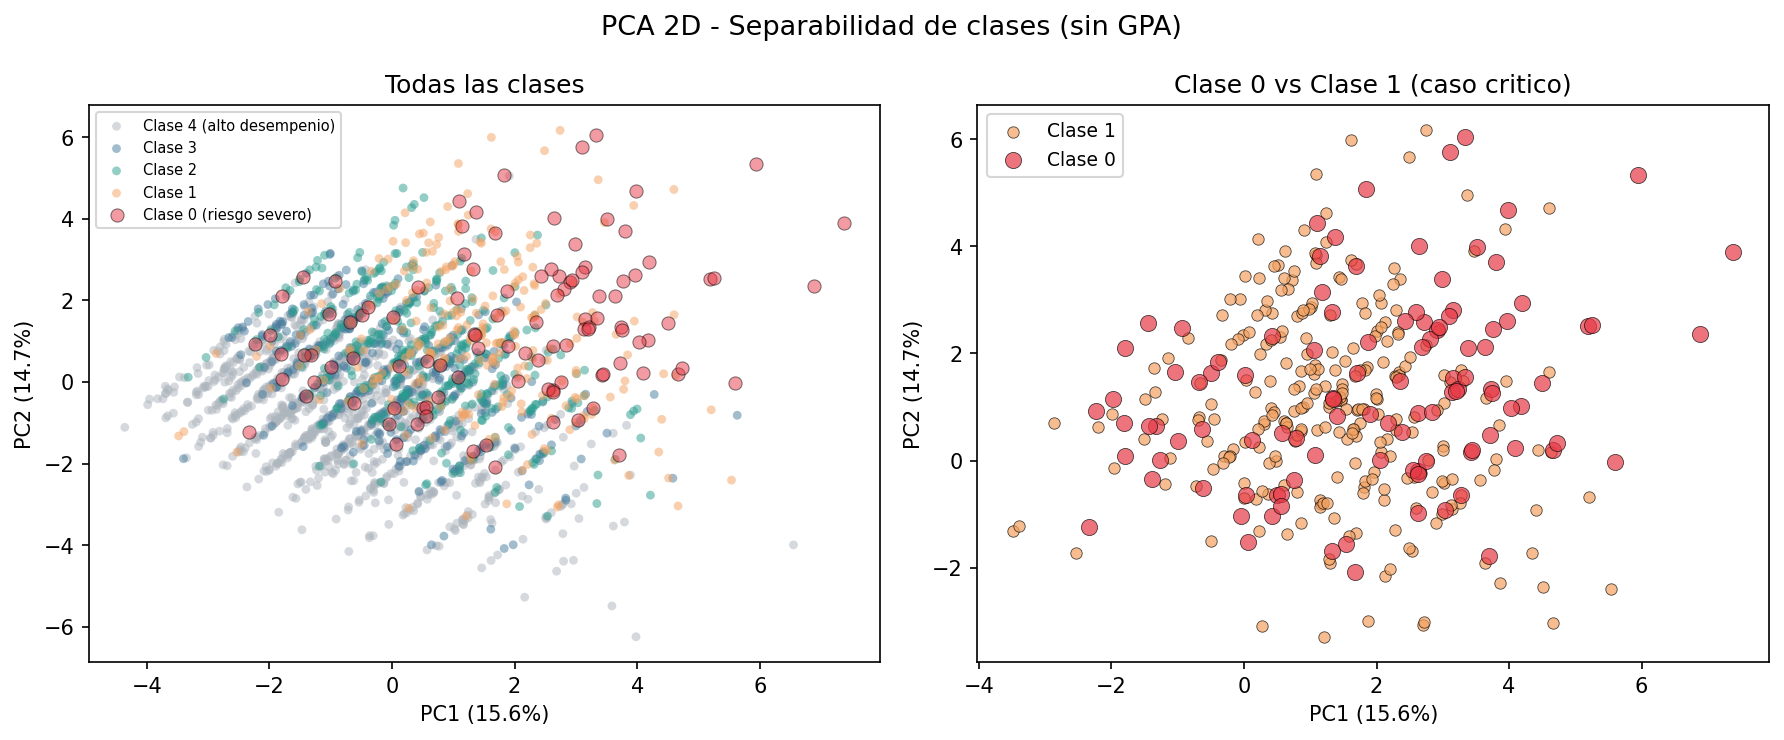
\includegraphics[width=0.95\linewidth]{separabilidad_pca.png}
\caption{Visualización en dos componentes principales de la separabilidad entre clases sin \texttt{GPA}.}
\label{fig:apendice_pca}
\end{figure}

La Figura~\ref{fig:apendice_pca} refuerza este hallazgo de forma
visual. Aunque la clase~0 presenta cierta tendencia a ocupar regiones
distintas del espacio proyectado, existe traslape considerable con la
clase~1. Esto explica por qué varios enfoques adicionales
(\textit{SMOTE}, clasificación ordinal, ajuste de umbrales, dos
etapas e incluso métodos alternativos como
\textit{HistGradientBoosting}) no lograron superar de manera
consistente al mejor \textit{Random Forest} con ingeniería de
variables.

\begin{figure}[!t]
\centering
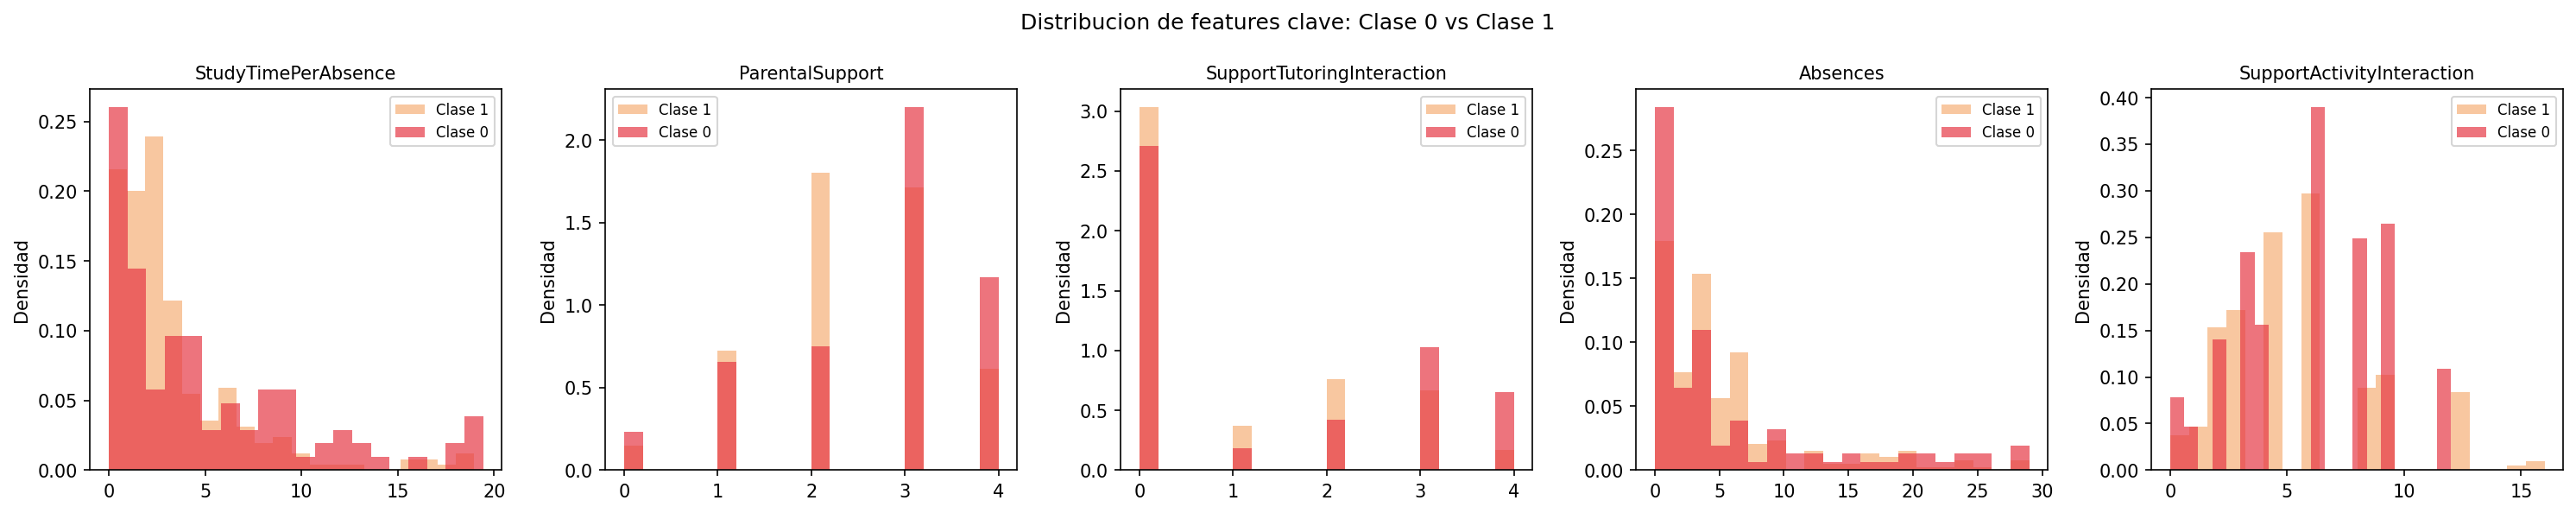
\includegraphics[width=0.95\linewidth]{separabilidad_distribuciones.png}
\caption{Distribuciones comparadas de las variables más separables entre clase 0 y clase 1.}
\label{fig:apendice_dists}
\end{figure}

Las distribuciones de la Figura~\ref{fig:apendice_dists} muestran el
mismo patrón desde otra perspectiva: hay diferencias observables, pero
no una separación tajante. En la evaluación binaria exclusiva entre
clase~0 y clase~1 se obtuvo un AUC de 0.7345, mientras que en el
escenario clase~0 contra todas las demás clases se obtuvo un AUC de
0.8211. Esta diferencia sugiere que la clase~0 sí es distinguible del
conjunto global, pero su frontera más problemática está precisamente
en la cercanía con la clase~1.

En consecuencia, el límite principal del escenario sin \texttt{GPA}
no parece estar únicamente en la arquitectura del clasificador, sino
en el nivel de solapamiento real entre perfiles de bajo desempeño y
desempeño inmediatamente superior. Este apéndice, por tanto, no solo
documenta un experimento alternativo, sino que ofrece una lectura más
institucional del problema: aun sin historial de calificaciones, los
atributos conductuales y de apoyo permiten recuperar señal relevante,
pero el techo de separabilidad del dataset impone una restricción
natural sobre la detección temprana del riesgo severo.

\phantomsection\label{sec:referencias}
\begin{thebibliography}{00}

\bibitem{ieeeaccess}
M. R. Islam, M. T. Islam, S. Nooruddin \textit{et al.},
``Student's performance analysis and prediction using deep learning,''
\textit{IEEE Access}, vol. 9, pp. 163949--163966, 2021,
doi: 10.1109/ACCESS.2021.3119596.

\bibitem{dropout}
N. Srivastava, G. Hinton, A. Krizhevsky, I. Sutskever y
R. Salakhutdinov, ``Dropout: A simple way to prevent neural networks
from overfitting,'' \textit{Journal of Machine Learning Research},
vol. 15, pp. 1929--1958, 2014. [En línea]. Disponible en:
\url{https://jmlr.org/papers/v15/srivastava14a.html}

\bibitem{rf_algorithms}
A. M. Rizk y A. M. El-Bakry, ``Using decision trees and random forest
algorithms to predict and determine factors contributing to first-year
university students' learning performance,'' \textit{Algorithms},
vol. 14, no. 11, art. 318, 2021. [En línea]. Disponible en:
\url{https://www.mdpi.com/1999-4893/14/11/318}

\bibitem{rf_dropout_review}
M. Costa e Silva, A. Fonseca y C. Leal, ``Supervised machine learning
algorithms for predicting student dropout and academic success: a
comparative study,'' \textit{Discover Education}, vol. 2, art. 79,
2023. [En línea]. Disponible en:
\url{https://link.springer.com/article/10.1007/s44163-023-00079-z}

\bibitem{rf_advising}
N. Altabraweh, A. Alshoshan, M. Medhat Gaber y otros, ``Predicting
Student Performance to Improve Academic Advising Using the Random
Forest Algorithm,'' \textit{International Journal of Distance
Education Technologies}, vol. 20, no. 1, 2022,
doi: 10.4018/IJDET.296702. [En línea]. Disponible en:
\url{https://www.sciencedirect.com/science/article/pii/S1539310022000047}

\bibitem{rf_mooc}
M. Ahad, M. Tripathi, S. Pathak y otros, ``Predicting Student Dropout
in Self-Paced MOOC Course Using Random Forest Model,''
\textit{Information}, vol. 12, no. 11, art. 476, 2021. [En línea].
Disponible en: \url{https://www.mdpi.com/2078-2489/12/11/476}

\bibitem{review_edm}
S. Alturki, ``Predicting Academic Outcomes: A Survey from 2007 Till
2018,'' \textit{Technology, Knowledge and Learning}, vol. 26,
pp. 291--304, 2021. [En línea]. Disponible en:
\url{https://link.springer.com/article/10.1007/s10758-020-09476-0}

\bibitem{review_success}
A. Shahiri, W. Husain y N. A. Rashid, ``A review on predicting
student's performance using data mining techniques,''
\textit{Procedia Computer Science}, vol. 72, pp. 414--422, 2015.
[En línea]. Disponible en:
\url{https://www.sciencedirect.com/science/article/pii/S1877050915036183}

\end{thebibliography}

\end{document}
